\documentclass{article}

\usepackage{arxiv}

\usepackage[utf8]{inputenc} % allow utf-8 input
\usepackage[T1]{fontenc}    % use 8-bit T1 fonts
\usepackage{lmodern}        % https://github.com/rstudio/rticles/issues/343
\usepackage{hyperref}       % hyperlinks
\usepackage{url}            % simple URL typesetting
\usepackage{booktabs}       % professional-quality tables
\usepackage{amsfonts}       % blackboard math symbols
\usepackage{nicefrac}       % compact symbols for 1/2, etc.
\usepackage{microtype}      % microtypography
\usepackage{graphicx}

\title{The Explainability of Time Series Downsampling}

\author{
    Morgan Frodsham
   \\
    School of Computing \\
    Newcastle University \\
  Newcastle upon Tyne, UK \\
  \texttt{\href{mailto:M.C.M.Frodsham2@newcastle.ac.uk}{\nolinkurl{M.C.M.Frodsham2@newcastle.ac.uk}}} \\
  }


% tightlist command for lists without linebreak
\providecommand{\tightlist}{%
  \setlength{\itemsep}{0pt}\setlength{\parskip}{0pt}}


% Pandoc citation processing
\newlength{\cslhangindent}
\setlength{\cslhangindent}{1.5em}
\newlength{\csllabelwidth}
\setlength{\csllabelwidth}{3em}
\newlength{\cslentryspacingunit} % times entry-spacing
\setlength{\cslentryspacingunit}{\parskip}
% for Pandoc 2.8 to 2.10.1
\newenvironment{cslreferences}%
  {}%
  {\par}
% For Pandoc 2.11+
\newenvironment{CSLReferences}[2] % #1 hanging-ident, #2 entry spacing
 {% don't indent paragraphs
  \setlength{\parindent}{0pt}
  % turn on hanging indent if param 1 is 1
  \ifodd #1
  \let\oldpar\par
  \def\par{\hangindent=\cslhangindent\oldpar}
  \fi
  % set entry spacing
  \setlength{\parskip}{#2\cslentryspacingunit}
 }%
 {}
\usepackage{calc}
\newcommand{\CSLBlock}[1]{#1\hfill\break}
\newcommand{\CSLLeftMargin}[1]{\parbox[t]{\csllabelwidth}{#1}}
\newcommand{\CSLRightInline}[1]{\parbox[t]{\linewidth - \csllabelwidth}{#1}\break}
\newcommand{\CSLIndent}[1]{\hspace{\cslhangindent}#1}

\usepackage{booktabs}
\usepackage{longtable}
\usepackage{array}
\usepackage{multirow}
\usepackage{wrapfig}
\usepackage{float}
\usepackage{colortbl}
\usepackage{pdflscape}
\usepackage{tabu}
\usepackage{threeparttable}
\usepackage{threeparttablex}
\usepackage[normalem]{ulem}
\usepackage{makecell}
\usepackage{xcolor}
\begin{document}
\maketitle


\begin{abstract}
Trusting data-driven decision-making goes beyond demonstrating
compliance with legal, regulatory and ethical obligations;
decision-makers also need to trust how the data is used. Handling,
storing and visualising the volume of data being generated today
requires data practitioners to make assumptions and processing choices
that remain opaque to decision-makers. Downsampling is an established
technique to select a representative subset of time series data that
preserves the original data shape while reducing the number of data
points in the time series. The research outlined by this paper explores
decision-makers' trust in data, data practitioners' experience of
communicating data insights to decision-makers, and a new visualisation
methodology for explaining the impact of downsampling on high-volume
time series data. It combines user research insights from interviews
with 16 UK Civil Servants with analysis of time series features for 900
imputed time series to identify and visualise the features that are most
sensitive to downsampling. This research shows the potential for
improving decision-makers' trust in data by helping data practitioners
to create transparency in the data processing pipeline, communicate the
impact of downsampling, and support conversations about which algorithms
or parameters are most appropriate for particular decision-maker use
cases.
\end{abstract}


\hypertarget{introduction}{%
\section{INTRODUCTION}\label{introduction}}

HM Government is committed to making data-driven decisions that engender
public trust
\protect\hyperlink{ref-data2017}{{[}1{]}}--\protect\hyperlink{ref-data2022}{{[}4{]}}.
Data-driven decisions are considered to be \emph{``more well-informed''}
\protect\hyperlink{ref-data2017}{{[}1{]}}, effective
\protect\hyperlink{ref-data2022}{{[}4{]}}, consistent
\protect\hyperlink{ref-data2021}{{[}3{]}}, and better at scale
\protect\hyperlink{ref-data2020}{{[}2{]}}. Despite this, there is a lack
of trust in government use of data
\protect\hyperlink{ref-trust}{{[}5{]}}. This suggests that public trust
in data-driven decisions goes beyond how the \emph{``data complies with
legal, regulatory and ethical obligations''}
\protect\hyperlink{ref-data2021}{{[}3{]}}. The UK public need to have
\emph{``confidence and trust in how data, including personal data, is
used''} \protect\hyperlink{ref-data2020}{{[}2{]}}, and this requires
transparency \protect\hyperlink{ref-trust}{{[}5{]}}.

To make data-driven decisions, it is likely that government
decision-makers' need transparency of how data is used to trust the data
insights they are presented with. Trust implies trusting which data
points are selected, how this data is collected and stored, and the
capability of data practitioners to understand the quality, insights and
limitations of it. At every stage of the data processing pipeline, data
practitioners have the opportunity to communicate the data impact of
assumptions and choices they are making. This could support
decision-makers in trusting the data informing their decisions while
helping decision-makers understand limitations of the data and
thresholds at which data insights can be relied upon for each decision.

The research shared in this paper explores this dynamic with a two
pronged approach. User research with 16 UK Civil Servants investigates
what helps decision-makers trust the data insights they are presented
with and how data practitioners assess, and communicate, the
trustworthiness of the data. These insights are combined with analysis
of how to explain the impact of downsampling algorithms on time series
data without detailing extensive statistical evidence.

Downsampling involves selecting a representative subset of data to
preserve its original shape while reducing the number of data points
\protect\hyperlink{ref-datapoint}{{[}6{]}},
\protect\hyperlink{ref-MinMaxLTTB}{{[}7{]}}. Time series data is used
throughout HM Government \protect\hyperlink{ref-pathway}{{[}8{]}} to
inform decision-makers across various domains
\protect\hyperlink{ref-onstool}{{[}9{]}}; it is also widely generated
and used by industry and research
\protect\hyperlink{ref-TVStore}{{[}10{]}}. However, the volume of time
series data is continuously increasingly
\protect\hyperlink{ref-datapoint}{{[}6{]}}, posing significant
challenges for handling and visualising this popular data type
\protect\hyperlink{ref-TVStore}{{[}10{]}}.

Data practitioners must use methods that reduce the quantity of data
(data volume) to align with limitations like processing time, computing
costs, storage capabilities, and sustainability ambitions
\protect\hyperlink{ref-TVStore}{{[}10{]}}--\protect\hyperlink{ref-Shift}{{[}12{]}}.
Downsampling is an established technique
\protect\hyperlink{ref-downsampling}{{[}13{]}},
\protect\hyperlink{ref-sampling}{{[}14{]}} for reducing data volumes.
Data reduction is vital for making voluminous time series understandable
for human observation \protect\hyperlink{ref-Sveinn}{{[}11{]}} and an
essential step in many time series database solutions
\protect\hyperlink{ref-datapoint}{{[}6{]}}. However, little attention
has been devoted to how downsampling impacts decision-makers trust in
the data. How to communicate the impact of downsampling algorithms on
time series data also remains understudied
\protect\hyperlink{ref-datapoint}{{[}6{]}},
\protect\hyperlink{ref-Sveinn}{{[}11{]}}.

Downsampling is an important part of how time series data is used and is
a technical issue whose impact, this research posits, is important for
decision-makers to understand. Downsampling expands the boundaries of
uncertainty and risk for decision-makers as data practitioners may not
realise the significance of the data being discarded. For example, it is
time and computing resource intensive to transport the terabytes of data
generated daily by offshore oil platforms
\protect\hyperlink{ref-CISCO}{{[}15{]}} without data discarding
techniques like downsampling \protect\hyperlink{ref-TVStore}{{[}10{]}}.
For decision-makers of platform safety and productivity, it is vital to
have this information as quickly as possible and understand how the
discarded data limits the insights they are considering. It is also
important for decision-makers looking at analysis of \(CO_2\) levels on
an open-plan office floor to decide how many officials can work in the
office each day post-Covid. Downsampling algorithms preserve different
data points \protect\hyperlink{ref-datapoint}{{[}6{]}},
\protect\hyperlink{ref-MinMaxLTTB}{{[}7{]}},
\protect\hyperlink{ref-Sveinn}{{[}11{]}}, which could change the risk
threshold for the decision-maker. In complex decisions, such choices
throughout the data pipeline may have cumulative or disproportionately
larger consequences later as their future ramifications are unlikely to
be fully understood \protect\hyperlink{ref-challenger}{{[}16{]}}. It is
important, therefore, that data practitioners are able to communicate
the impact of choices made throughout the data pipeline.

This paper shares initial insights from user research on
decision-makers' trust in how data is used and suggests a visualisation
methodology for communicating the impact of downsampling algorithms on
time series. This methodology combines user research insights with R
packages \texttt{imputeTS} \protect\hyperlink{ref-imputeTS_R}{{[}17{]}}
and \texttt{Rcatch22} \protect\hyperlink{ref-catch22_R}{{[}18{]}} to
identify time series features that are most sensitive to downsampling
and visualise the impact of different downsampling algorithms on these
features. It is hoped this will improve how data practitioners
communicate the impact of downsampling, support conversations about
which algorithms or parameters are most appropriate for particular use
cases, and increase decision-makers' trust in data by creating
transparency in the data processing pipeline.

\hypertarget{related-work}{%
\section{RELATED WORK}\label{related-work}}

This section provides an overview of previous related work to create a
clear understanding of the most relevant fields for this research and
identify the gaps being addressed by the paper.

\textbf{2.1 Data transparency}

Technology transparency, including institutional data practices, is
sociopolitical in nature
\protect\hyperlink{ref-political_transparency}{{[}19{]}}. There is a
growing number of researchers reflecting on society's transparency needs
\emph{``in terms of what is made transparent, for whom, how, when and in
what ways, and, crucially, who decides''}
\protect\hyperlink{ref-social_transparency}{{[}20{]}}.

The implicit assumption behind calls for transparency is that
\emph{``seeing a phenomenon creates opportunities and obligations to
make it accountable''} and, therefore, to change it
\protect\hyperlink{ref-transparency_lack}{{[}21{]}}. However, without
sufficient agency to explore the information being shared, seeing a
phenomenon often results in information overload that obfuscates or
diverts attention
\protect\hyperlink{ref-transparency_obfuscation}{{[}22{]}}. Without
agency, transparency is increasingly considered to be a fallacy
\protect\hyperlink{ref-transparency_fallacy}{{[}23{]}}.

Meaningful transparency is only realised when the information is
provided with the tools to transform access into agency
\protect\hyperlink{ref-transparency_lack}{{[}21{]}},
\protect\hyperlink{ref-transparency_fallacy}{{[}23{]}}. This suggests
that data practitioners simply communicating the assumptions and choices
made throughout the data processing pipeline to decision-makers is not
likely to create trust in how the data is used. Instead, data
practitioners should be encouraged to find tools, such as interactive
visualisations \protect\hyperlink{ref-datapoint}{{[}6{]}}, that put
agency into the hands of decision-makers.

\textbf{2.2 Time series visualisation}

Time series data is commonly visualised as a line graph
\protect\hyperlink{ref-Sveinn}{{[}11{]}},
\protect\hyperlink{ref-timenotes}{{[}24{]}},
\protect\hyperlink{ref-timetuner}{{[}25{]}}. Line graphs help the human
eye to observe only the most important data points
\protect\hyperlink{ref-Sveinn}{{[}11{]}} by conveying the overall shape
and complexity of the time series data
\protect\hyperlink{ref-datapoint}{{[}6{]}},
\protect\hyperlink{ref-downsampling}{{[}13{]}}. The most effective time
series visualisations are, however, interactive
\protect\hyperlink{ref-timenotes}{{[}24{]}}--\protect\hyperlink{ref-plotly}{{[}26{]}},
turning access into agency
\protect\hyperlink{ref-transparency_fallacy}{{[}23{]}} by allowing the
user to access details on demand. Evaluation of time series
visualisation is, therefore, a growing field of research
\protect\hyperlink{ref-timenotes}{{[}24{]}}.

However, this growing field of research does not extend to
visualisations of choices and assumptions made during the data
processing pipeline. Indeed, such visualisations are often a side effect
of research. This is exemplified by the R package \texttt{imputeTS}
\protect\hyperlink{ref-imputeTS_R}{{[}17{]}} where the impact of
imputation choices made by the user is only visualised to support users
through the complete process of replacing missing values in time series
\protect\hyperlink{ref-imputeTS}{{[}27{]}},
\protect\hyperlink{ref-missingdata}{{[}28{]}}. The research set out in
this paper harnesses the capabilities of \texttt{imputeTS} and its
`process' visualisations to help data practitioners communicate the
impact of downsampling choices made in the data processing pipeline.

\textbf{2.3 Value preserving data aggregation}

Technological innovation has generated an unprecedented amount of time
series data and this data volume continues to grow
\protect\hyperlink{ref-data2020}{{[}2{]}},
\protect\hyperlink{ref-TVStore}{{[}10{]}},
\protect\hyperlink{ref-storage}{{[}29{]}},
\protect\hyperlink{ref-CatchUp}{{[}30{]}}. For example, tackling climate
change is the UK Government's \emph{``number one international
priority''} \protect\hyperlink{ref-IR}{{[}31{]}}, yet climate
simulations that help inform decision-makers generate tens of terabytes
per second \protect\hyperlink{ref-TVStore}{{[}10{]}},
\protect\hyperlink{ref-climate}{{[}32{]}}. Value preserving data
aggregation (a subset of downsampling) algorithms play an important role
in addressing how this voluminous data is processed, stored
\protect\hyperlink{ref-TVStore}{{[}10{]}}, and visualised
\protect\hyperlink{ref-Sveinn}{{[}11{]}},
\protect\hyperlink{ref-dashql}{{[}33{]}} by minimising the computing
resources needed \protect\hyperlink{ref-TVStore}{{[}10{]}}, reducing
network latency, and improving rendering time
\protect\hyperlink{ref-datapoint}{{[}6{]}},
\protect\hyperlink{ref-MinMaxLTTB}{{[}7{]}}.

Value preserving data aggregation algorithms preserve the original data
points that are considered to best represent the original data. This
research uses two of the simplest algorithms: \emph{EveryNth}
\protect\hyperlink{ref-EveryNth}{{[}34{]}} and \emph{Percentage Change}
\protect\hyperlink{ref-boxcar}{{[}35{]}}. Descriptions of commonly used
value preserving data aggregation algorithms are provided in the table
below \protect\hyperlink{ref-datapoint}{{[}6{]}},
\protect\hyperlink{ref-MinMaxLTTB}{{[}7{]}},
\protect\hyperlink{ref-Sveinn}{{[}11{]}},
\protect\hyperlink{ref-dashql}{{[}33{]}}--\protect\hyperlink{ref-M4}{{[}37{]}}:

\renewcommand{\arraystretch}{1.5}

\begin{table}[H]

\caption{\label{tab:unnamed-chunk-1}Example Downsampling Algorithms}
\centering
\begin{tabular}[t]{>{\raggedright\arraybackslash}p{1.8in}|>{\raggedright\arraybackslash}p{3.8in}}
\hline
Algorithm & Description\\
\hline
EveryNth & Selects every nth data point.\\
\hline
Percentage Change & Selects every data point beyond a specified percentage of the previous data point.\\
\hline
Mode-Median Bucket & Selects mode or median within equally sized data buckets.\\
\hline
Min-Std-Error-Bucket & Selects data points with standard error of the estimate (SEE) in linear regression.\\
\hline
MinMax & Preserves minimum and maximum data points in each data bucket.\\
\hline
M4 & Selects the first and last as well as the minimum and maximum data points.\\
\hline
Longest-Line Bucket & Calculates line length (euclidean distance) between data buckets and selects one point per bucket which forms the longest total
line length through all the buckets.\\
\hline
Largest Triangle Three Bucket (LTTB) & Calculates the largest triangular surface between the previously selected data point and the average value of the next data bucket to select the highest point.\\
\hline
MinMaxLTTB & Preselects data points using MinMax before applying LTTB.\\
\hline
\end{tabular}
\end{table}

Data practitioners have recently made advances in the performance and
evaluation of downsampling approaches
\protect\hyperlink{ref-datapoint}{{[}6{]}},
\protect\hyperlink{ref-MinMaxLTTB}{{[}7{]}},
\protect\hyperlink{ref-downsampling}{{[}13{]}},
\protect\hyperlink{ref-sampling}{{[}14{]}},
\protect\hyperlink{ref-plotly}{{[}26{]}},
\protect\hyperlink{ref-dashql}{{[}33{]}}--\protect\hyperlink{ref-MinMaxOrdered}{{[}36{]}}.
These advances focus on the effectiveness of the algorithm in delivering
downsampled data that represents the original data as accurately as
possible. This is a vital part of enabling and improving data-driven
decision-making, but it is focused on supporting data practitioners in
their data analysis. Instead, the research set out in this paper aims to
support data practitioners to communicate the impact of their
downsampling choices for decision-makers.

\textbf{2.4 Time series feature analysis}

The increasing sizes of modern time series data sets have also generated
new research into the characteristics of time series
\protect\hyperlink{ref-catch22}{{[}38{]}}. These characteristics are
often used to identify features that enable efficient clustering and
classification of time series data, especially for machine learning. A
comprehensive library of such features is the highly comparative time
series analysis \texttt{hctsa} toolbox. This shares the 4791
high-performing features after computationally comparing thousands of
characteristics from across scientific time series analysis literature
\protect\hyperlink{ref-fulcher2017}{{[}39{]}}.

Utilising such a library, however, is computationally expensive
\protect\hyperlink{ref-catch22}{{[}38{]}}. C. H. Lubba et. al have
attempted to address this by identifying a subset of 22 features (as
well as mean and standard deviation) that are tailored to time series
data mining tasks \protect\hyperlink{ref-catch22}{{[}38{]}},
\protect\hyperlink{ref-bagnall}{{[}40{]}}, which are shared in the
\texttt{Rcatch22} R package. Although further research is needed to
evaluate the relative performance of different feature sets on different
types of problems, the \texttt{catch22} features performs well against
other feature libraries across 800 diverse real-world and
model-generated time series \protect\hyperlink{ref-henderson}{{[}41{]}}.

Features used to classify time series data could provide a common
framework by which to consistently compare different downsampling
algorithms and parameters. The research set out in this paper utilises
the \texttt{Rcatch22} subset of features to explore impact of
downsampling and create a visual process for explaining this impact.

\hypertarget{user-research}{%
\section{USER RESEARCH}\label{user-research}}

Interviews with 16 UK Civil Servants (nine decision-makers and seven
data practitioners) highlight the importance of transparency in enabling
data-driven decision-making across government. This section outlines how
the user research is designed and the key insights it generated.

\textbf{3.1 Design}

User research produced over 16 hours of recorded and transcribed
interviews with decision-makers and data practitioners (the outputs are
confirmed in Annex A). These interviews are hosted virtually on MS
Teams, instead of in-person, to enable recording and transcription; this
creates the potential to move beyond qualitative thematic analysis and
implement alternative techniques, such as natural language processing.
Interviews are selected over surveys because concepts like transparency
and trust are complex and nuanced. One-to-one interviews are selected
instead of focus groups to minimise authority bias and potential
groupthink.

Like many interview studies \protect\hyperlink{ref-futzing}{{[}42{]}},
the participants for this user research are selected by contacting
relevant individuals in the researcher's professional network. This
introduces bias as the sample of participants is neither representative
nor drawn from the overall population. This could engender confirmation,
false consensus and group think biases as these participants are likely
to operate in the same professional bubble, which would skew the
insights generated by this user research. To mitigate further biases,
two interview scripts are used; one for all decision-makers and the
other for all data practitioners. However, it is important to note that
follow-up questions vary to ease the flow of each interview and help
participants share further detail in their responses.

Qualitative analysis is conducted on the content of each interview to
understand the themes and identify quotes that reflect the participant's
sentiments. This is combined with natural language processing keyword
extraction. The python libraries \texttt{docx} and \texttt{nltk} are
used to import and clean the interview text data; capitalisation,
`stopwords,' and words with three or fewer letters are removed.
Interviews are anonymised as the time stamps, interviewer name and
participant name are removed \protect\hyperlink{ref-jono}{{[}43{]}};
text data from the interviewer is also removed so that natural language
processing is only conducted on participant responses. Limited natural
language processing is then applied by tokenising the remaining words
and counting the number of each unique word. These word counts alongside
the qualitative thematic analysis inform concept maps
\protect\hyperlink{ref-GPT}{{[}44{]}} which aim to show the key themes
and words.

\textbf{3.2 Insights}

Transparency of data provenance, collection, and the analysis pipeline
is clearly desired by decision-makers to understand the reliability,
repeatability, and quality of the data they're presented with. All
interviewed decision-makers and data-practitioners shared that this is
best communicated through engaging conversations and interactive
visualisations. Both decision-makers and data practitioners emphasised
the importance of communicating the story behind data, its assumptions,
and how the data changes through time. Everyone interviewed acknowledged
that this is difficult to achieve and how to improve this is a topic of
live debate.

Insights from this user research indicate that decision-makers desire a
spectrum of transparency for decisions. This spectrum depends on the
question being addressed by the data: it's complexity, importance and
potential impact. To trust the data informing data-driven decisions,
decision-makers and data practitioners repeatedly request transparency
of the data context, source and limitations as well as an assessment of
overall confidence in the data.

Quotes from the decision-maker interviews highlight that decision-makers
find it difficult to develop the correct views of \emph{``how much they
can trust the data''}. They address their desire for more emphasis on
the \emph{``metadata and how to appropriately describe the level of
uncertainty and provenance of the data''} to help ensure the data is
being applied to the context it was collected for. They share the
importance of understanding if \emph{``there is anything that is baked
into what is being provided''} in order to trust the data and, how the
source of this trust changes as data practitioners become
decision-makers because they rarely see the raw data and so \emph{``have
to have an understanding of what preprocessing has been done, because it
almost always has been {[}done{]}''}. Decision-makers share that
visualisations are important for conveying \emph{``specific insights
that simply looking at numbers can't get over''} and emphasise that if
analysts \emph{``clearly explain what the limitations are and rigorously
present that, then I'll trust {[}the analysis{]} more''}. Quotes from
data practitioner interviews are shared in Annex B.

Figure 1 below shares example concept maps outlining the key themes from
two anonymised decision-maker and data-practitioner interviews. All the
interview concept maps are shared in Annex C; only summative content
from these interviews is presented in compliance with the consent forms
signed by the user research participants.

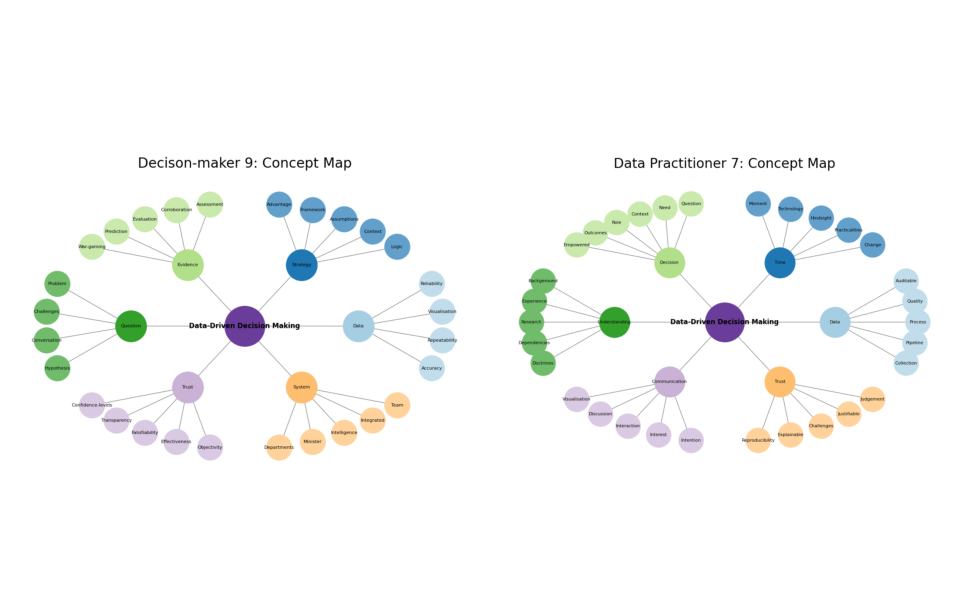
\includegraphics{210431461_CSC8639_Dissertation_files/figure-latex/ConceptMapExample-1.pdf}
\vspace{-3.3cm}

The findings from this user research indicate that decision-makers need
transparency of how the data is used to trust the insights informing
data-driven decisions. This suggests that endeavours to create greater
transparency in data pipelines, such as the research outlined in the
subsequent sections of this paper, are worthy of further study. It also
suggests that evaluating the objectivity and quality of data sources as
well as mechanisms to develop common descriptions of data insight
uncertainty or confidence-levels are potential avenues for data science
to have greater policy impact.

It is important to reiterate that the findings of this user research are
limited and, potentially, biased. Given the consistency of insights from
the user research participants, it is clear that further interviews with
a wider, random subset of the decision-maker and data practitioner
populations in HM Government would be beneficial.

\hypertarget{analysis-methodology}{%
\section{ANALYSIS METHODOLOGY}\label{analysis-methodology}}

This section outlines the analysis design undertaken to identify and
communicate the impact of downsampling algorithms on time series data
without extensive statistical evidence.

\textbf{4.1 Data}

The eight Alan Turing Institute \texttt{Annotated\ Change}
\protect\hyperlink{ref-ATIChangePoint}{{[}45{]}} synthetic time series
are selected for initial analysis. These are selected because they are
cleaned time series from a reputable institution with known change
points that are designed to provide examples of different types of time
series. However, there is an inherent limitation in using synthetic time
series for analysis because the data has been generated for a different
purpose. These synthetic time series (`100,' `200,' `300,' `400,' `500,'
`600,' `700,' `800') are used in demonstrations to support change point
annotators annotate real-world data sets for the
\texttt{Turing\ Change\ Point\ Data\ set}
\protect\hyperlink{ref-ATIChangePoint}{{[}45{]}}. The eighth
\texttt{Annotated\ Change} synthetic time series (`800') is multivariate
and thus split in two (`800A' and `800B') to create nine synthetic time
series for this research and enable better comparison. The nine time
series are visualised in Annex D.

\textbf{4.2 Downsampling}

These synthetic time series are imported into \texttt{RStudio} from
\texttt{JSON} scripts and two downsampling algorithms are applied to all
with the \texttt{Jettison\ MVP\ Code}
\protect\hyperlink{ref-Jettison}{{[}46{]}}. This enables initial
insights into the impacts of downsampling with minimally complex code.
The two algorithms used by the \texttt{Jettison\ MVP\ Code}
\protect\hyperlink{ref-Jettison}{{[}46{]}} are \emph{EveryNth}, which
selects every \(n\) data points, and \emph{Percentage Change}, which
selects every data point that has greater than \(n\) percent difference
between the last transmitted and newest values.

The \texttt{Jettison\ MVP\ Code}
\protect\hyperlink{ref-Jettison}{{[}46{]}} applies these algorithms
iteratively across each of the nine synthetic time series. This creates
parameters 1 to 50 for each downsampling algorithm and
\texttt{Annotated\ Change} time series. There are now 900 time series
for investigation, 450 for each downsampling algorithm.

The R package \texttt{imputeTS}
\protect\hyperlink{ref-imputeTS_R}{{[}17{]}} is applied to all 900 time
series to obtain the remaining data volume after downsampling, number of
missing values (NAs), and number of gaps in the time series. This is
important to understand the effect of each downsampling algorithm.
Initial analysis highlights that the effect of each downsampling
algorithm is unevenly distributed across the 50 parameters; for example,
\emph{EveryNth} discards data more quickly than \emph{Percentage Change}
so comparing the time series for each parameter is insufficient. The
remaining data volume, therefore, provides a common variable that
enables like-for-like comparison between the downsampling algorithms and
their impact.

The missing values for each of the 900 time series are replaced by the
\texttt{imputeTS} linear interpolation function. This is a simple
imputation algorithm that returns each time series to its original
length and is a commonly used approach to present line graphs
\protect\hyperlink{ref-compressiontech}{{[}47{]}}. Returning the time
series to their original length enables a like-for-like comparison of
downsampling impact. For each \texttt{Annotated\ Change} synthetic time
series, there is now an imputed time series for parameters 1 to 50 and
each downsampling algorithm.

\textbf{4.3 Features}

The \texttt{Rcatch22} package
\protect\hyperlink{ref-catch22_R}{{[}18{]}} enables the computation of a
value for each of the \texttt{catch22} time series features
\protect\hyperlink{ref-catch22}{{[}38{]}}. Values for the 24 time series
features are calculated for each of the nine original time series and
900 imputed time series. The difference between the original and imputed
feature values is calculated and that difference is scaled, dividing by
the standard deviation with the \texttt{scale()} R function, to
accurately compare how the downsampling algorithms impact these
\texttt{catch22} features. The coefficient of variation across the 900
imputed time series for each \texttt{catch22} feature is also calculated
to indicate and compare the sensitivity of each feature to downsampling.
The \texttt{catch22} features are considered to be more sensitive if
their coefficient of variation across the 900 imputed time series is
higher.

It is important to note that the \texttt{catch22} time series features
reflect characteristics that help cluster and classify different time
series, they are not selected for their impact on downsampling. This
analysis could be taken further by statistically investigating whether
features sensitive to downsampling are equally applicable to all time
series types.

\textbf{4.4 Visualisation}

Combining \texttt{imputeTS} \protect\hyperlink{ref-imputeTS_R}{{[}17{]}}
and \texttt{Rcatch22} \protect\hyperlink{ref-catch22_R}{{[}18{]}} in
this way is unstudied. Initial visual analysis to observe the impact of
downsampling on \texttt{catch22} features is conducted by using bar and
line graphs alongside heatmaps. All the decision-makers interviewed as
part of the user research stressed the importance of visualisation in
data transparency and data-driven decision-making. In line with this,
different approaches to visualising the impact of downsampling are tried
to explore how the impact of downsampling could best be visually
communicated by data practitioners. The visualisations created by this
research are under-developed and would benefit from usability research
to ensure they meet the aim of this research.

\hypertarget{results-and-evaluation}{%
\section{RESULTS AND EVALUATION}\label{results-and-evaluation}}

\vspace{-0.4cm}

This section shares and discusses the results of this research,
identifying their limitations and potential avenues for further
investigation. These results are presented in three themes: downsampling
sensitivity, downsampling impact, and feature variation.

\newpage

\textbf{5.1 Downsampling sensitivity}

Seven \texttt{catch22} features show a wider dispersion across the 900
imputed time series than the other 15 features. These seven features are
considered to be more sensitive to the impacts of downsampling. To
demonstrate the sensitivity of these seven features, features with the
highest absolute coefficient of variation values across all the imputed
time series are visualised in the bar graph below. The absolute
coefficient of variation values for all 24 features is shared in Annex
E.

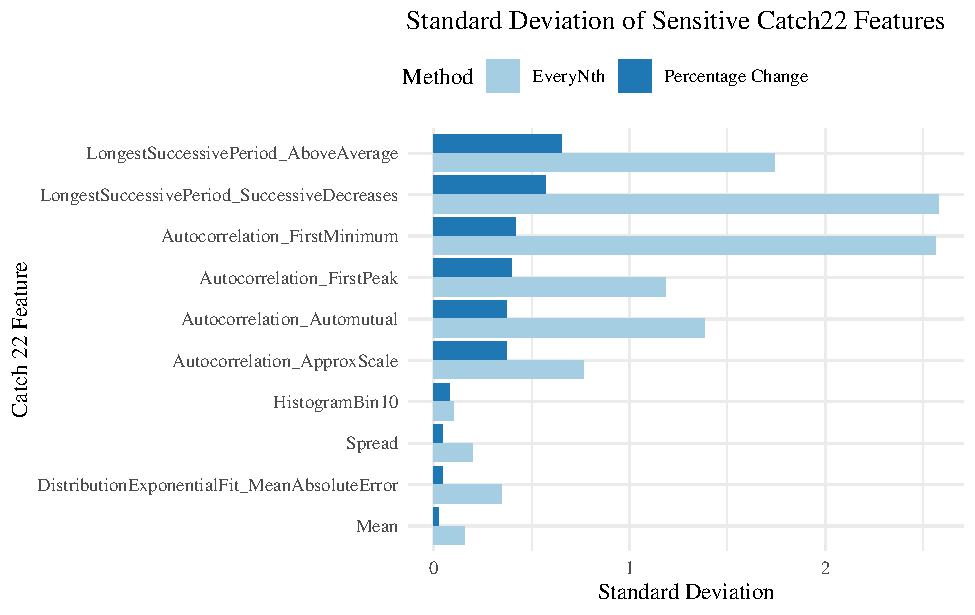
\includegraphics{210431461_CSC8639_Dissertation_files/figure-latex/CombinedSensitivity-1.pdf}

Figure 2 suggests that the \emph{Percentage Change} algorithm impacts
the \texttt{catch22} time series features more than the \emph{EveryNth}
algorithm. This is surprising as the \emph{EveryNth} algorithm discards
more data, more quickly, in the 50 parameters of downsampling. The
sensitivity of these features to the \emph{Percentage Change} algorithm
is worthy of further statistical analysis to understand why it impacts
the feature's coefficient of variation values more. It would also be
beneficial to investigate the impact of \emph{Percentage Change} further
by creating downsampling parameters beyond 50 until the same volume of
data is discarded by both algorithms.

The absolute coefficient of variation values for the seven most
sensitive \texttt{catch22} features, rounded to to two decimal points,
are presented in table 2.

\vspace{-0.2cm}

\begin{table}[H]

\caption{\label{tab:unnamed-chunk-2}Coefficient of Variation for the Seven Most Sensitive Catch22 Features}
\centering
\begin{tabular}[t]{l|r|r|r}
\hline
Feature & everyNth & Percentage Change & Combined\\
\hline
LongestPeriod\_Decreases & 0.99 & 1.58 & 1.47\\
\hline
Autocorr\_FirstMinimum & 0.65 & 0.77 & 1.18\\
\hline
Autocorr\_Automutual & 0.71 & 0.88 & 1.14\\
\hline
LongestPeriod\_AboveAverage & 0.70 & 1.37 & 1.12\\
\hline
Autocorr\_ApproxScale & 0.78 & 0.72 & 0.97\\
\hline
Autocorr\_FirstPeak & 0.64 & 0.99 & 0.96\\
\hline
DistributionExponentialFit\_MAE & 0.79 & 0.18 & 0.74\\
\hline
\end{tabular}
\end{table}

The combined absolute coefficient of variation values are used to
identify the seven \texttt{catch22} features that appear to be most
sensitive. Table 2 shows that the longest sequence of successive steps
that decrease \protect\hyperlink{ref-feature_book}{{[}48{]}}
(\texttt{LongestPeriod\_Decrease} or
\texttt{SB\_BinaryStats\_diff\_longstretch0}) has the highest combined
sensitivity.

These results indicate that it may be possible to communicate the impact
of downsampling via the sensitivity of the \texttt{catch22} features.
This analysis could be taken further by examining whether the
coefficient of variation is the best measure of sensitivity and
investigating whether the changes in the \texttt{catch22} features is
directly caused by the impact of downsampling.

\textbf{5.2 Downsampling Impact}

Identifying that seven \texttt{catch22} features appear to be more
sensitive to the impacts of downsampling enables data practitioners to
evaluate and communicate the impact of different downsampling algorithms
without deep statistical analysis. The difference between the values of
\texttt{catch22} features for the nine original time series and 900
imputes time series is used to measure the impact of downsampling.
Figure 3 below visualises this difference scaled (divided by the
standard deviation) for the seven most sensitive \texttt{catch22}
features across the 900 imputed time series and each of the 50
parameters.

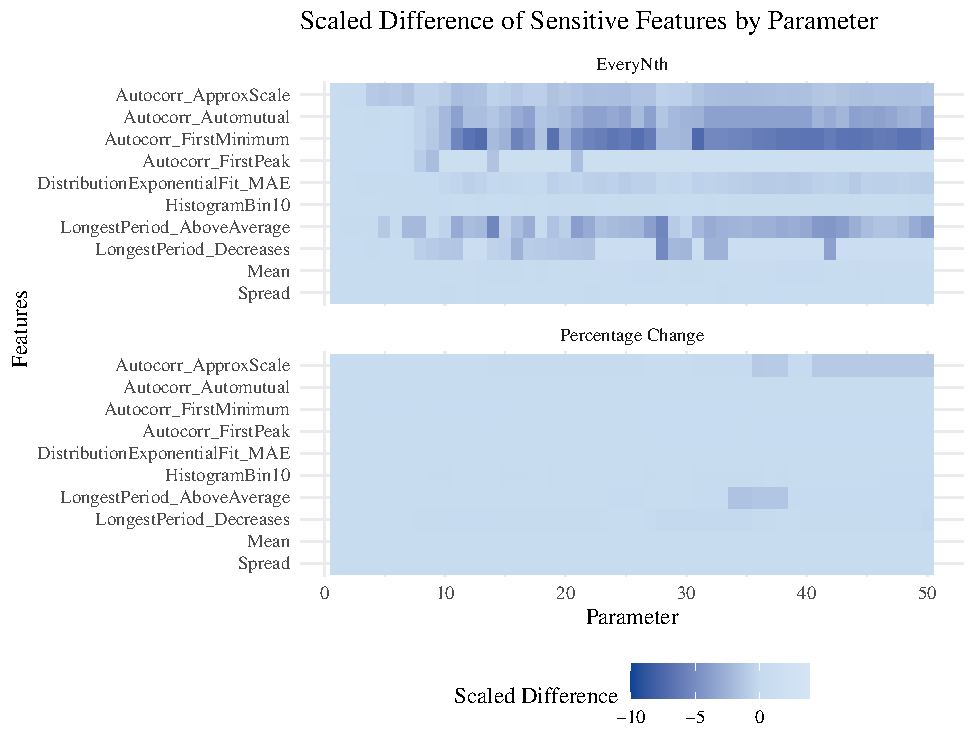
\includegraphics{210431461_CSC8639_Dissertation_files/figure-latex/Heatmap_param-1.pdf}

Figure 3 suggests that the approximate scale of autocorrelation
(\texttt{Autocorr\_ApproxScale} or \texttt{CO\_f1ecac}) and the longest
sequence of successive values greater than the mean
(\texttt{LongestPeriod\_AboveAverage} or
\texttt{SB\_BinaryStats\_mean\_longstretch1}) are the first
\texttt{catch22} features to be impacted by the downsampling algorithms.
Interestingly, Figure 3 also demonstrates that the feature values
impacted by both downsampling algorithms tend to increase in comparison
the original values. This warrants further investigation.

However, the parameters prevent a like-for-like comparison of the two
downsampling algorithms as \emph{EveryNth} discards data more quickly
than \emph{Percentage Change}. Figure 4 on the next page also visualises
the scaled difference between the values of the original
\texttt{catch22} features and the imputed time series, but across the
volume of data retained by the downsampling algorithms before
\texttt{imputeTS} \protect\hyperlink{ref-imputeTS_R}{{[}17{]}} imputes
the missing values.

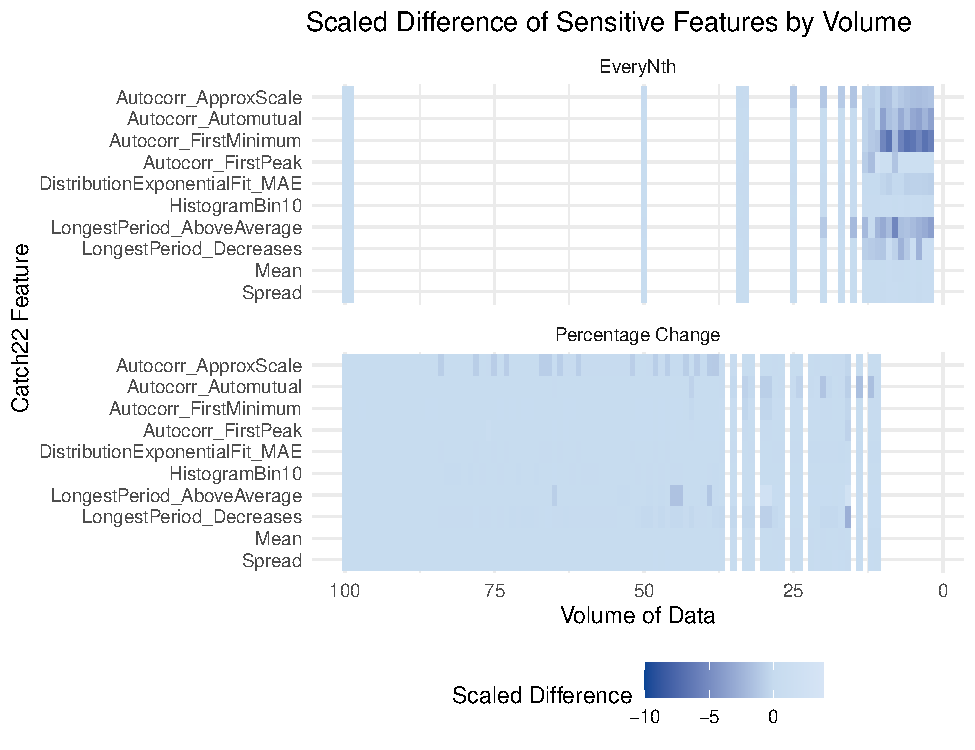
\includegraphics{210431461_CSC8639_Dissertation_files/figure-latex/Heatmap_vol-1.pdf}

Figure 4 demonstrates that data volume retained by the downsampling
algorithms creates acute differences, especially when fewer than 20 data
points remain after \emph{EveryNth} is applied. However we cannot
conclude that there is a significant difference between the algorithms
over and above the volume of data remaining without further
investigation. Interestingly, the impact of \emph{Percentage Change}
appears to be inconsistent; there are some retained data volumes where
\texttt{Autocorr\_ApproxScale} and \texttt{LongestPeriod\_AboveAverage}
do not appear to be impacted by \emph{Percentage Change} even though
larger retained data volumes appear to be impacted. This also warrants
further investigation.

Downsampling can perturb the statistical properties
\protect\hyperlink{ref-ATIChangePoint}{{[}45{]}} and visual perception
\protect\hyperlink{ref-graphsampling}{{[}49{]}} of data.
\texttt{Catch22} features are statistical properties of time series. It
is likely that some of these statistical properties will be more or less
affected by downsampling because downsampling algorithms preserve
different data points from the original time series. A full table of the
statistical properties represented by each \texttt{catch22} feature is
shared in Annex F.

It is not possible, however, to understand the impact of both
downsampling algorithms from this visualisation. The \emph{Percentage
Change} algorithm needs to be applied for more than 50 parameters so
that it discards volumes of data comparable to the \emph{EveryNth}
algorithm. Despite this, the heatmap visualisation of downsampling
impact holds potential; Figure 4 suggests that, with the same volume of
data, the downsampling algorithms impact the \texttt{catch22} features
differently.

\textbf{5.3 Feature Variation}

The impact of both downsampling algorithms on the most sensitive
features appears to vary across different time series types. This is
exemplified by the \texttt{catch22} feature
\texttt{LongestPeriod\_Decreases}
(\texttt{SB\_BinaryStats\_diff\_longstretch0}), which calculates the
longest sequence of successive steps in the time series that decrease
\protect\hyperlink{ref-feature_book}{{[}48{]}}. The feature has the
highest coefficient of variation across the 900 time series; the line
graphs in Figure 5 on the next page share the differences between the
\texttt{catch22} feature value of the original time series and the 50
time series imputed from these after downsampling; these differences are
scaled for better comparisons. The title of each line graph refers to
the original nine synthetic time series (for example, `100,' `200,' and
`300').

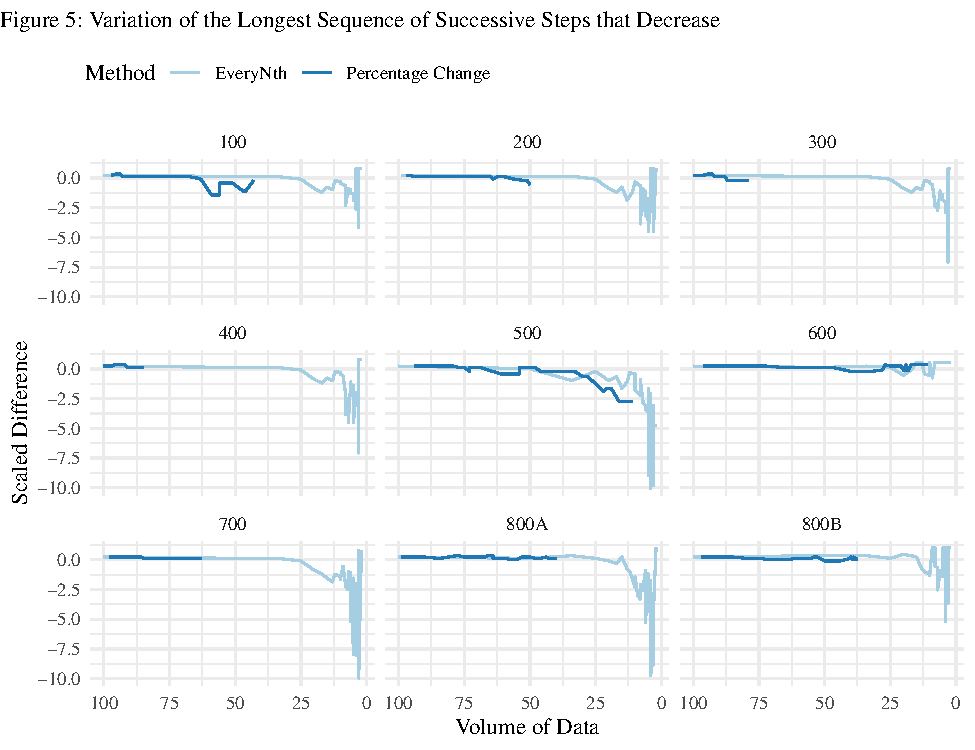
\includegraphics{210431461_CSC8639_Dissertation_files/figure-latex/LongestDecreases-1.pdf}

Figure 5 presents the impact of discarding data for both downsampling
algorithms. The volume of data retained by the \emph{Percentage Change}
algorithm varies by the type of time series whereas the data volume
retained by the \emph{EveryNth} algorithm trends towards zero. The line
graphs presented in Figure 5 highlight how different downsampling
algorithms may more or less preserve the integrity of different time
series. For example, time series `100,' `300,' `500' and `800B' appear
to be more impacted by the Percentage Change algorithm than other time
series. How the most sensitive \texttt{catch22} time series features
vary across the different time series types is shared in Annex G.

This variation of downsampling algorithms across time series types
causes the author to question whether the downsampling sensitivity of
\texttt{catch22} features may vary across time series type too. An
example of this dynamic is visualised by the line graphs in Figure 6 on
the next page, which plot the scaled difference of the six most
sensitive \texttt{catch22} features for time series `500.' Time series
`500' was selected as more data is discarded by the \emph{Percentage
Change} algorithm, offering a better comparison.

Figure 6 on the next page highlights that, although
\texttt{LongestPeriod\_Decrease} is identified as the most sensitive
across both downsampling algorithms, \texttt{Autocorr\_Automutual}
(\texttt{IN\_AutoMutualInfoStats\_40\_gaussian\_fmmi}) might better
indicate the impact for time series `500.' \texttt{Autocorr\_Automutual}
is the minimum of the automutual information function; this
\texttt{catch22} feature outputs a measure of \emph{``autocorrelation in
the time series, as the minimum of the automutual information
function''} \protect\hyperlink{ref-feature_book}{{[}48{]}}.
\texttt{Autocorr\_FirstMinimum} (\texttt{CO\_FirstMin\_ac}) and
\texttt{Autocorr\_FirstPeak} (\texttt{PD\_PeriodicityWang\_th0\_01})
also seem to show early impacts of the \emph{Percentage Change}
algorithm.

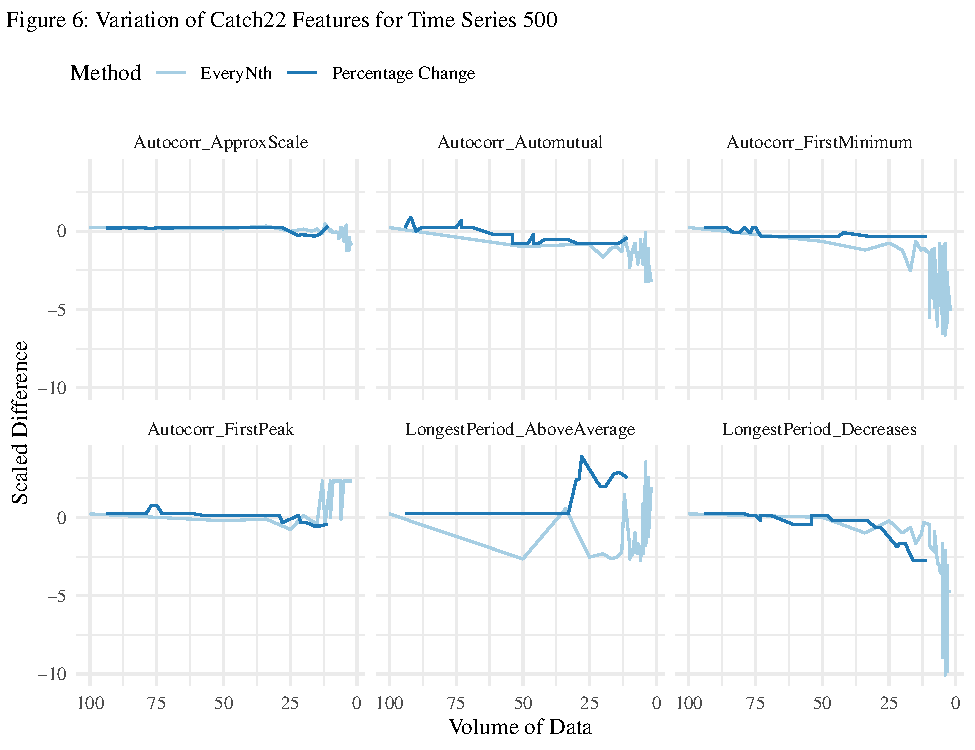
\includegraphics{210431461_CSC8639_Dissertation_files/figure-latex/Catch22Variation-1.pdf}

Interestingly, Figure 6 shows that the \emph{Percentage Change}
algorithm has the opposite impact on
\texttt{LongestPeriod\_AboveAverage}
(\texttt{SB\_BinaryStats\_mean\_longstretch1}) than the \emph{EveryNth}
algorithm.

A comparison of the most sensitive features for each time series type is
shared in Annex H. It would be beneficial to explore this further as the
variation may offer data practitioners a method for identifying subsets
of features that best indicate the preservation of different time
series.

\hypertarget{conclusion}{%
\section{CONCLUSION}\label{conclusion}}

Increasing volumes of time series data are being widely generated and
used by industry and research \protect\hyperlink{ref-TVStore}{{[}10{]}}.
Downsampling is a vital data processing technique for reducing this
volume, addressing limitations like processing time, computing costs,
storage capabilities and sustainability ambitions
\protect\hyperlink{ref-TVStore}{{[}10{]}}--\protect\hyperlink{ref-Shift}{{[}12{]}}.
However, downsampling can perturb the statistical properties
\protect\hyperlink{ref-ATIChangePoint}{{[}45{]}} and visual perception
\protect\hyperlink{ref-graphsampling}{{[}49{]}} of time series,
potentially impacting the insights that inform data-driven decisions.

Interviews with 16 UK Civil Servants (nine decision-makers and seven
data practitioners) highlight the importance of transparency in enabling
data-driven decision-making across government. Decision-makers shared
that there is a spectrum of transparency desired for the data processing
pipeline, which depends on the question being addressed by the data;
it's complexity, importance and potential impact. To trust the data
informing data-driven decisions, decision-makers and data practitioners
repeatedly requested transparency of the data context, source and
limitations as well as an assessment of overall confidence in the data.
This user research indicates that decision-makers need transparency of
how the data is used to trust the insights informing data-driven
decisions.

There are seven \texttt{catch22} time series features
\protect\hyperlink{ref-catch22}{{[}38{]}} that appear to be more
sensitive to the impacts of downsampling. \texttt{Catch22} features are
statistical properties of time series so they are more or less affected
by downsampling depending on which data points are preserved from the
original time series. The impact of the \emph{EveryNth} and
\emph{Percentage Change} downsampling algorithms on the most sensitive
features appears to vary across different time series types. The
downsampling sensitivity of \texttt{catch22} features also appears to
differ across time series. These results suggest that different subsets
of \texttt{catch22} features could be selected to best indicate the
preservation of time series after downsampling. Tailored subsets of
features enable data practitioners to design and build interactive
visualisations that create transparency of the data processing pipeline
for decision-makers to explore the limitations of the data they are
considering.

The varying sensitivity of \texttt{catch22} features to different
downsampling algorithms is previously unstudied. This research offers a
new visualisation methodology for data practitioners to communicate the
impact of downsampling on different decisions and create meaningful
transparency about the downsampling choices they are making throughout
the data processing pipeline. This could help decision-makers to trust
the data informing their decisions, supporting decision-makers to
understand the limitations of the data available, and the thresholds at
which the data insights can or cannot be relied upon for each decision.

\hypertarget{future-work}{%
\section{FUTURE WORK}\label{future-work}}

There are many avenues for future work to better understand the
findings, and address the limitations, of this research.

\textbf{6.1 User research}

Further user with a wider, more representative group of decision-makers
and data practitioner is needed to develop statistically significant
findings for HM Government. Alongside this, additional analysis on the
transcripts and recordings of the user research would improve the
analysis. For example, using other natural language processing
techniques, such as topic modelling, to better identify the connections
between the key themes identified. Usability research with
decision-makers and data practitioners would also beneficial. Usability
would contribute to the refinement of visualisations so that they better
communicate the impact of downsampling on different time series. How
these visualisations perturb the decision-makers' and data
practitioners' perception of downsampling impact is an important avenue
of further investigation
\protect\hyperlink{ref-graphsampling}{{[}49{]}}.

\textbf{6.2 Downsampling Sensitivity}

It would be beneficial to use the data pipeline developed by C. H. Lubba
et. al \protect\hyperlink{ref-catch22}{{[}38{]}} to generate other
subsets of time series features for distinct tasks in different domains.
Examining the downsampling sensitivity of new subsets of
\texttt{catch22} features is likely to generate the information needed
to understand why certain features are more sensitive to downsampling
across different types of time series. It could also be interesting to
explore the impact of data discarding techniques, such as downsampling,
through classifications of missing data
\protect\hyperlink{ref-missingdata}{{[}28{]}}. Such classifications may
offer alternative features for evaluating and visualising the impact of
discarding data.

\textbf{6.3 Downsampling Impact}

Further iterations of downsampling on the synthetic time series used in
this research is an important step to address the limitations of this
research. These iterations will enable a better comparison of the
\emph{EveryNth} and \emph{Percentage Change} algorithms. Equally,
repeating the analysis methodology of this research for other
downsampling algorithms, such as LTTB
\protect\hyperlink{ref-MinMaxLTTB}{{[}7{]}},
\protect\hyperlink{ref-Sveinn}{{[}11{]}},
\protect\hyperlink{ref-MinMaxOrdered}{{[}36{]}}, as well as applying
this method to the real-world time series shared by the
\texttt{Alan\ Turing\ Change\ Point\ Dataset}
\protect\hyperlink{ref-ATIChangePoint}{{[}45{]}} set will allow a deeper
investigation into the impact of downsampling. These avenues of future
work are also vital for generating the information needed to fully
realise the ambitions of this research - developing comparative and
interactive visualisations to better communicate the impact of
downsampling on time series.

\textbf{6.4 Feature Variation}

The future work for understanding downsampling sensitivity and impact
could be combined to develop thresholds and benchmarks for different
time series. This avenue for further investigation could enable the most
relevant and sensitive time series features to be embedded for proactive
downsampling that reduces the demand on computing resources. For
example, embedding the most sensitive features in smart sensors
monitoring a particular type of time series would enable better
downsampling at the point of collection, reducing demand on computing
resources for storage. Such tailoring of downsampling could also
facilitate more nuanced discussions between decision-makers and data
practitioners on the thresholds of downsampling for different decision
types to ensure that insights from downsampled data are used within the
bounds of their limitations.

\newpage

\hypertarget{annex-a-acknowledgement-of-user-research}{%
\section{Annex A: Acknowledgement of User
Research}\label{annex-a-acknowledgement-of-user-research}}

In line with the signed consent forms, the user research transcripts and
unprocessed findings cannot be shared beyond the researcher and their
supervisor. Figure 7 shares the supervisor's email confirmation
acknowledging the user research conducted.

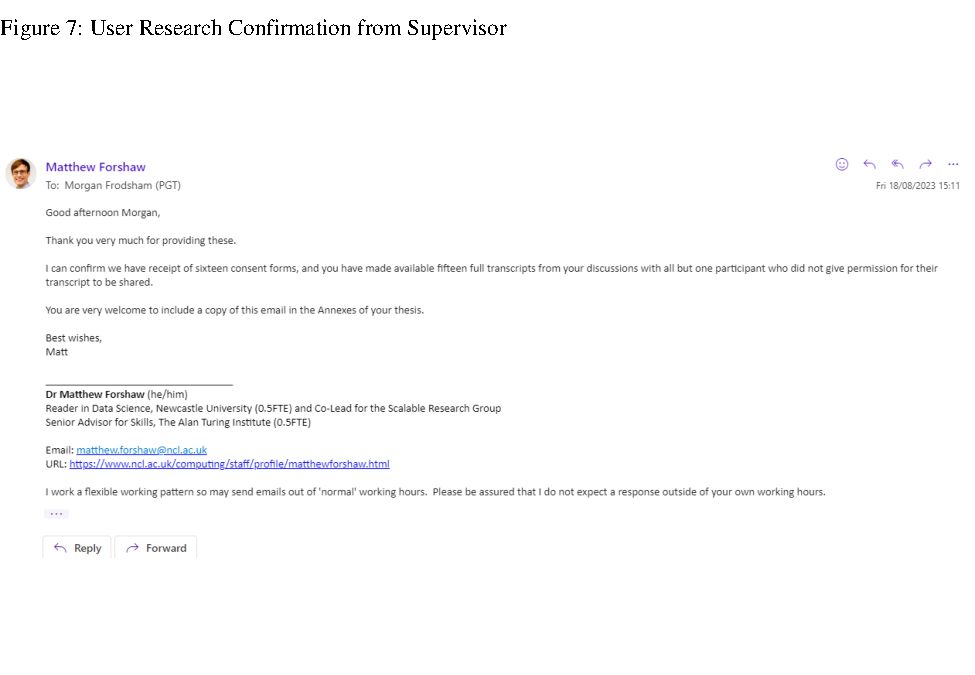
\includegraphics[width=1\linewidth]{210431461_CSC8639_Dissertation_files/figure-latex/unnamed-chunk-3-1}
\newpage

\hypertarget{annex-b-data-pracitioner-quotes}{%
\section{Annex B: Data Pracitioner
Quotes}\label{annex-b-data-pracitioner-quotes}}

Interesting (anonymised) quotes that highlight the sentiment of data
practitioners from user research interviews are shared below:

\begin{itemize}
\item
  \emph{``You come at it from a particular viewpoint with your
  particular expertise, somebody with different background, somebody
  with different expertise might come at the problem in a different
  way.''}
\item
  \emph{``\ldots my impression is that a lot of people make decisions
  from data without actually understanding what that data represents or
  simultaneously, and what the theoretical assumptions on our data and
  data collection is.''}
\item
  \emph{``\ldots getting the point across of how downsampling and other
  techniques effects that data getting that balance right of explaining
  the assumptions and explaining what what's been done without getting
  in the technical details\ldots{}''}
\item
  \emph{``I would probably think about the impact of the decision and
  that would inform me about whether I'm comfortable making a decision
  on that with that data.''}
\item
  \emph{``\ldots we have to understand what things you may think of the
  data tells you, but it doesn't actually tell you because that's where
  you often get caught out.''}
\item
  \emph{``\ldots making the assumption of what people how people will
  think the data will be interpreted versus how you can interpret the
  data is a really, really useful because you go, OK, people gonna want
  to say this about this data, but this is what actually sets.''}
\item
  \emph{``\ldots if you have done the due diligence, generally decision
  makers trust you to do the due diligence.''}
\item
  \emph{``The best that you can say in general is that you have to
  understand what the information requirement is and what the
  information processing is that happens, and then you can make an
  estimate of the effect that downsampling, or indeed any information
  reduction technique has on the on the decision.''}
\item
  \emph{``\ldots ensure that people are thinking about what the
  processes that they are going through in order to make the decision,
  not so, not just taking the recommendation but actually understanding
  how it's got there and where the data came from and how that was
  achieved.''}
\item
  \emph{``I think {[}helping decision-makers trust data{]} is quite
  dependent on the personality of who you're dealing with at the time
  and what they're willing to kind of expose of their own understanding
  and lack of understanding or motivation.''}
\item
  \emph{``Data is collected for a purpose then being used for another
  purpose and they might not exactly map on top of one another, which I
  think is quite challenging. Often we end up getting data that was
  collected by somebody else for something else, and we've got to
  shoehorn it into what we are interested in.''}
\item
  \emph{``I haven't engaged with stakeholders on a level like that to
  understand whether they are aware of the impacts of decisions like
  that on any end results and how much of a difference that can
  make\ldots{} but it is very much a stakeholder problem because it
  impacts what you will get out of it.''}
\end{itemize}

\newpage

\hypertarget{annex-c-user-research-concept-maps}{%
\section{Annex C: User Research Concept
Maps}\label{annex-c-user-research-concept-maps}}

\vspace{-0.4cm}

Key word counts alongside the qualitative thematic analysis inform
concept maps which visualise the key themes and key words. The concept
maps for each decision-maker and data practitioner interview are shared
in this section.

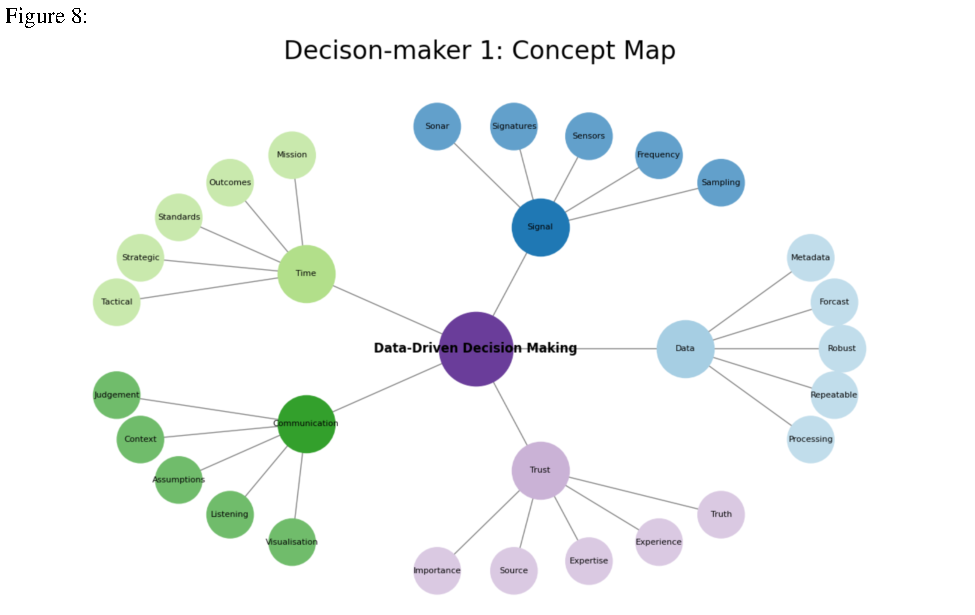
\includegraphics{210431461_CSC8639_Dissertation_files/figure-latex/unnamed-chunk-4-1.pdf}

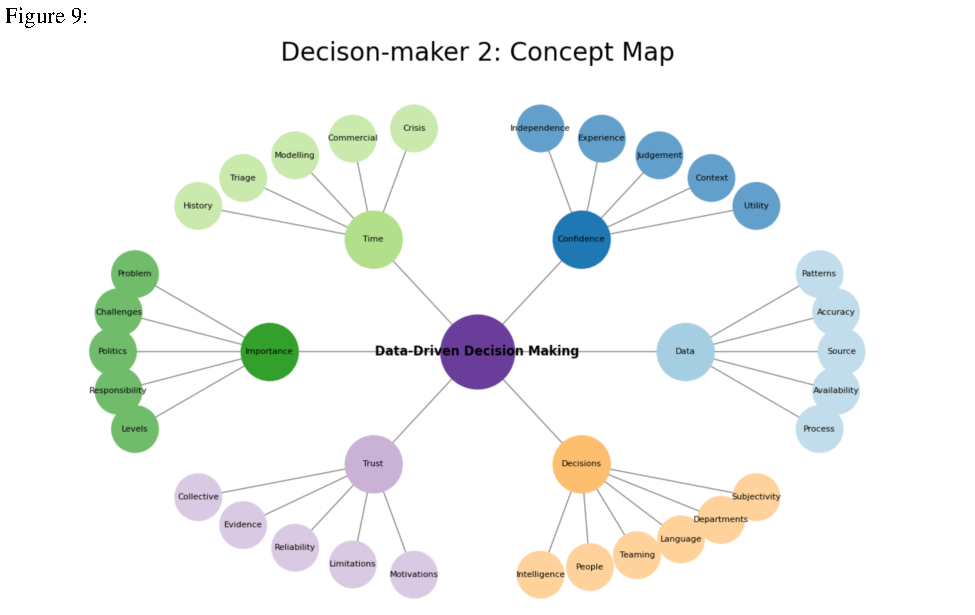
\includegraphics{210431461_CSC8639_Dissertation_files/figure-latex/unnamed-chunk-5-1.pdf}

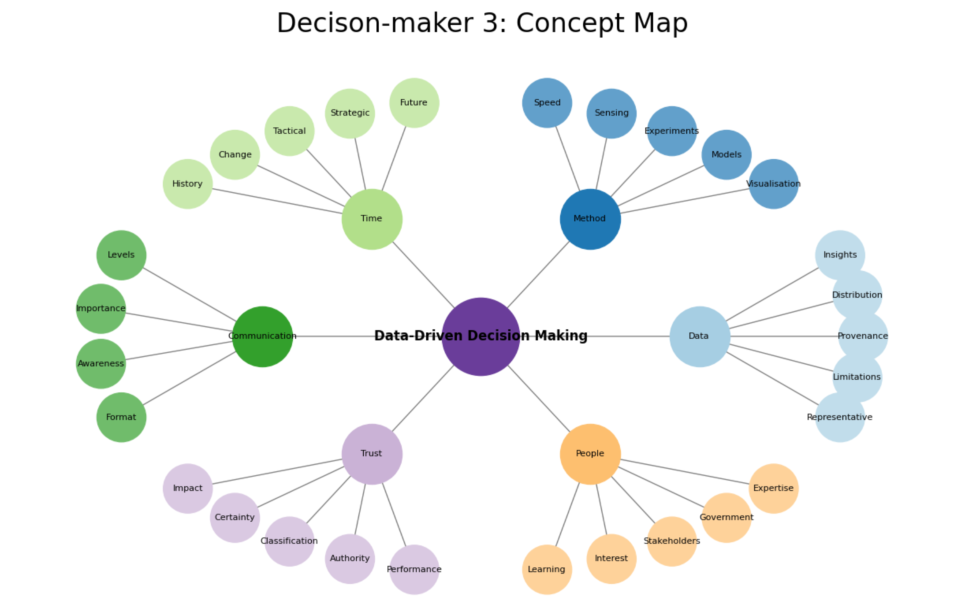
\includegraphics{210431461_CSC8639_Dissertation_files/figure-latex/unnamed-chunk-6-1.pdf}

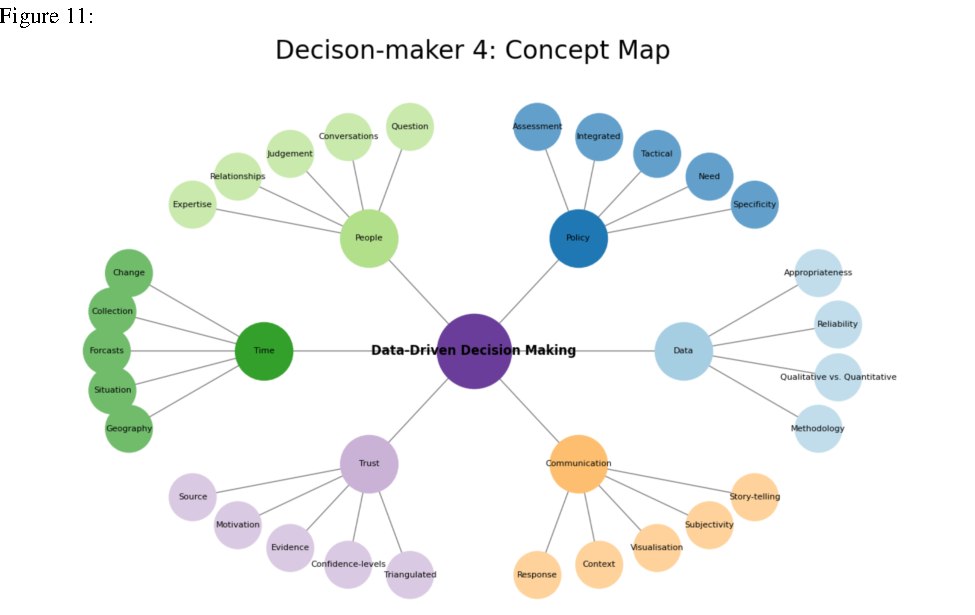
\includegraphics{210431461_CSC8639_Dissertation_files/figure-latex/unnamed-chunk-7-1.pdf}

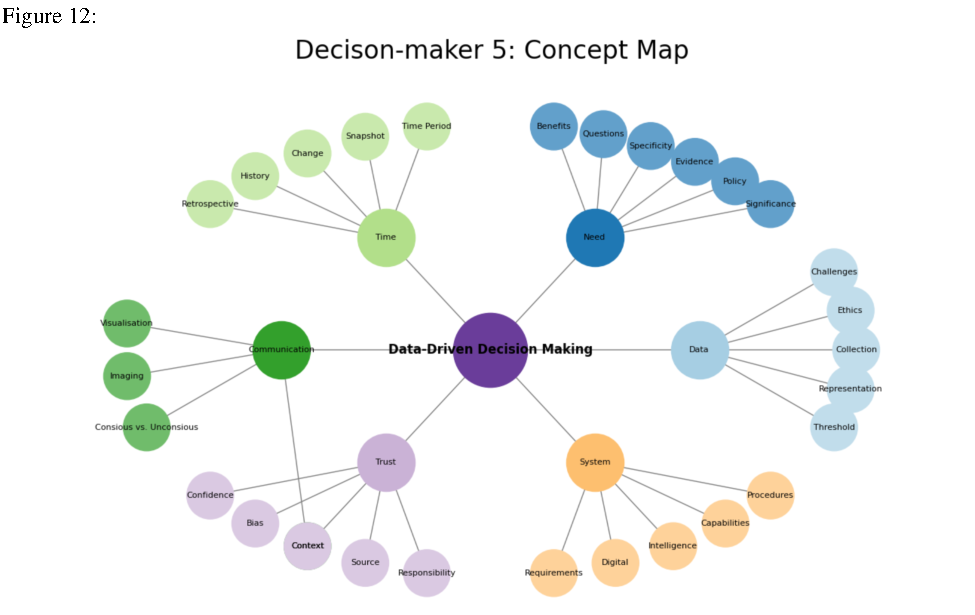
\includegraphics{210431461_CSC8639_Dissertation_files/figure-latex/unnamed-chunk-8-1.pdf}

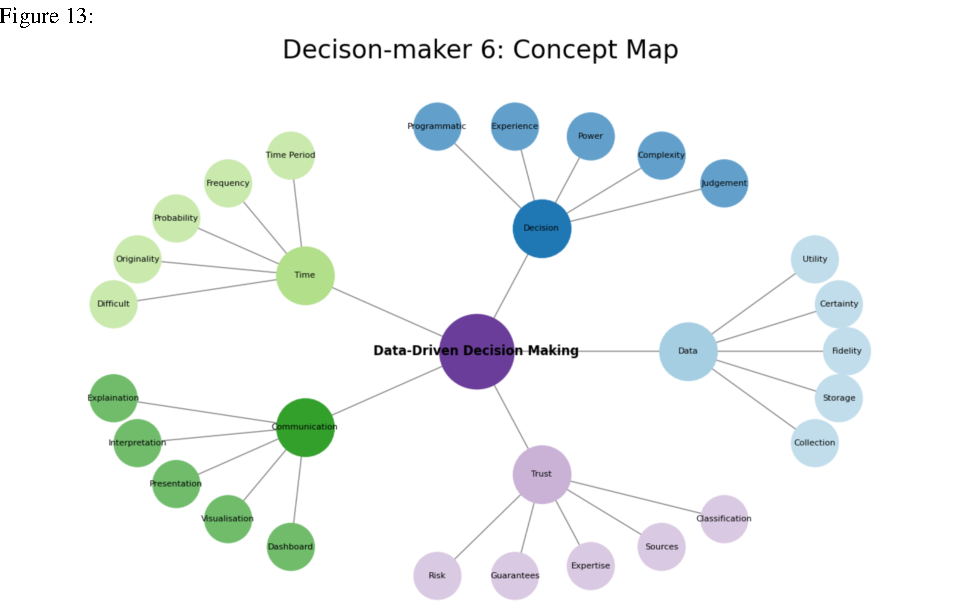
\includegraphics{210431461_CSC8639_Dissertation_files/figure-latex/unnamed-chunk-9-1.pdf}

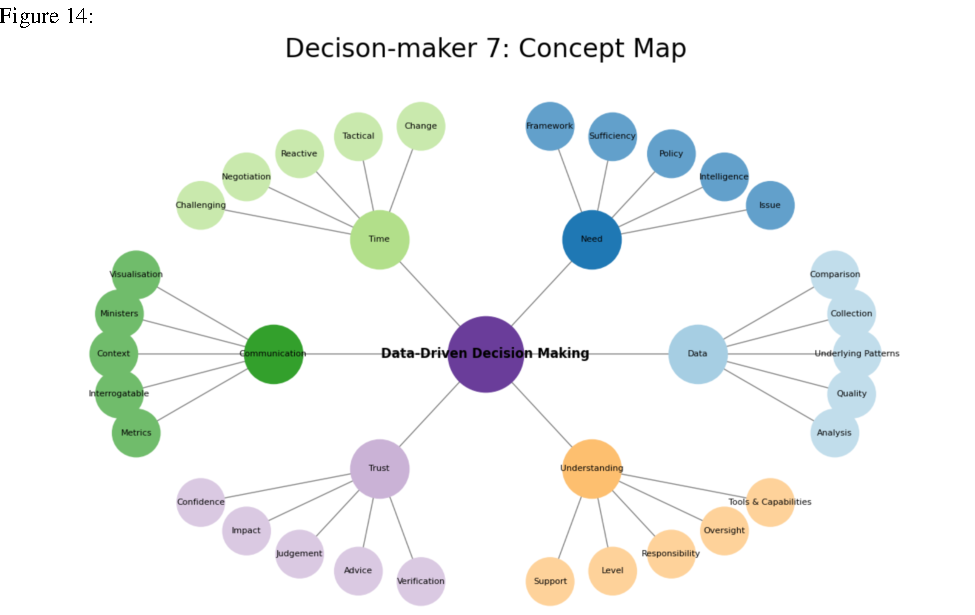
\includegraphics{210431461_CSC8639_Dissertation_files/figure-latex/unnamed-chunk-10-1.pdf}

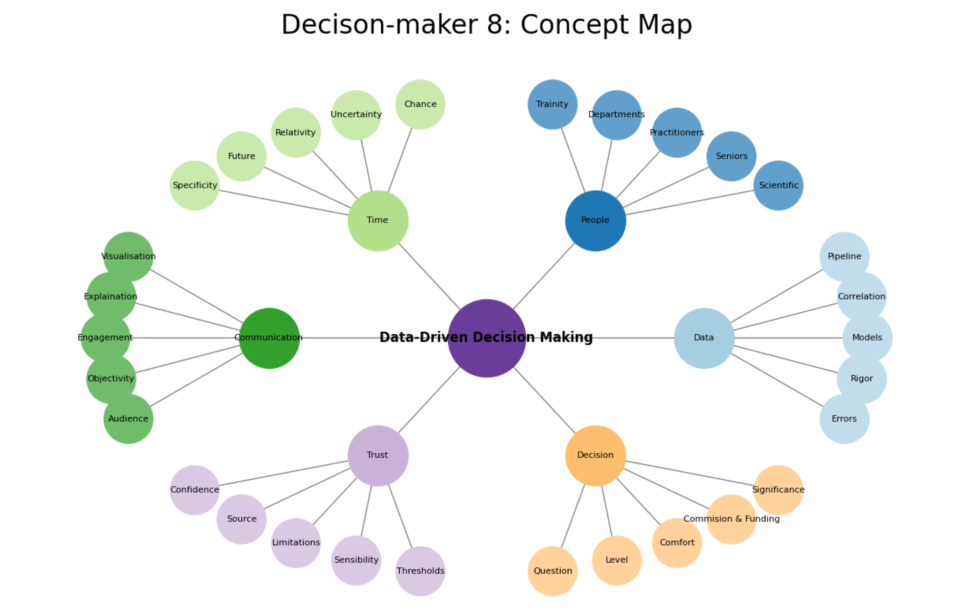
\includegraphics{210431461_CSC8639_Dissertation_files/figure-latex/unnamed-chunk-11-1.pdf}

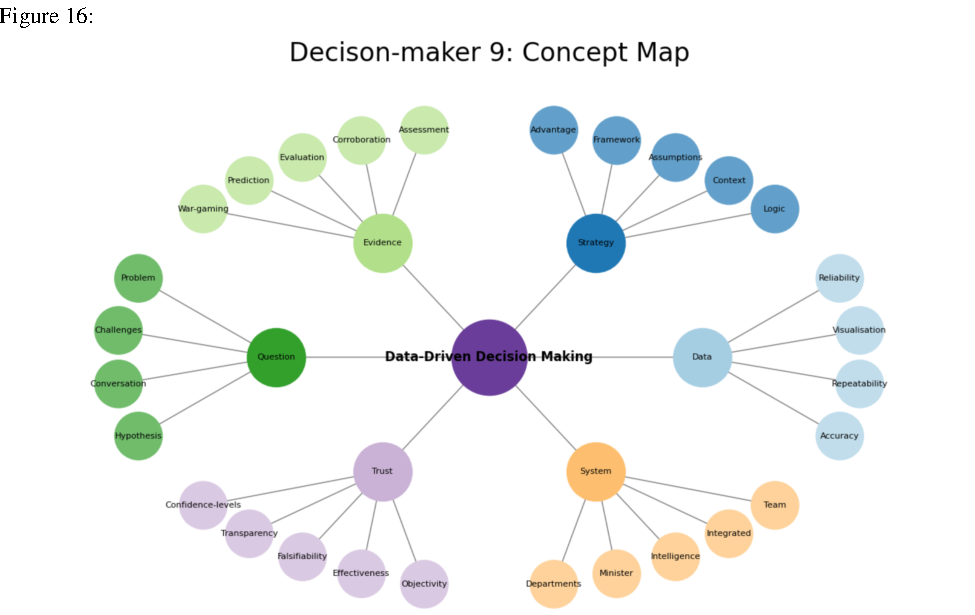
\includegraphics{210431461_CSC8639_Dissertation_files/figure-latex/unnamed-chunk-12-1.pdf}

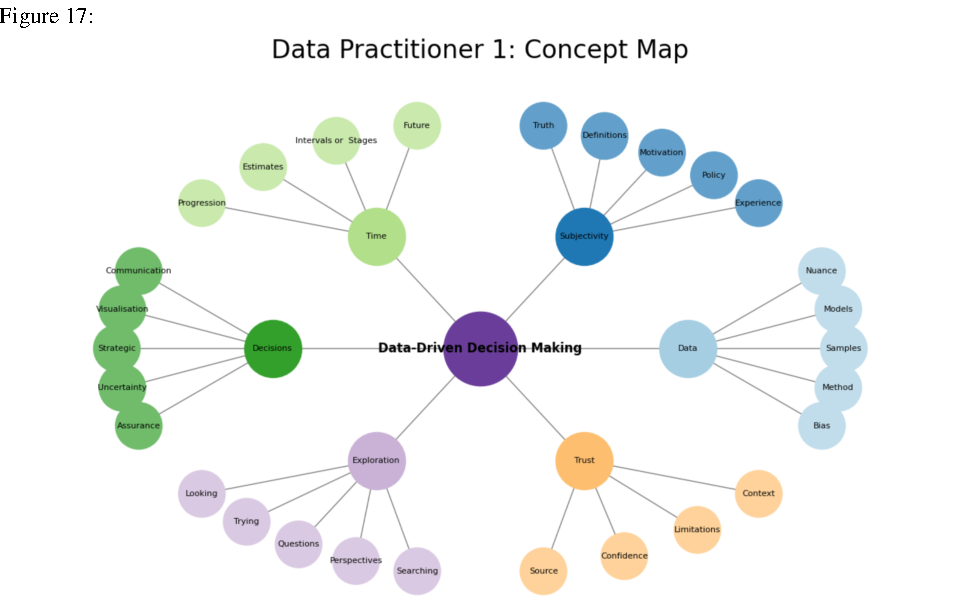
\includegraphics{210431461_CSC8639_Dissertation_files/figure-latex/unnamed-chunk-13-1.pdf}

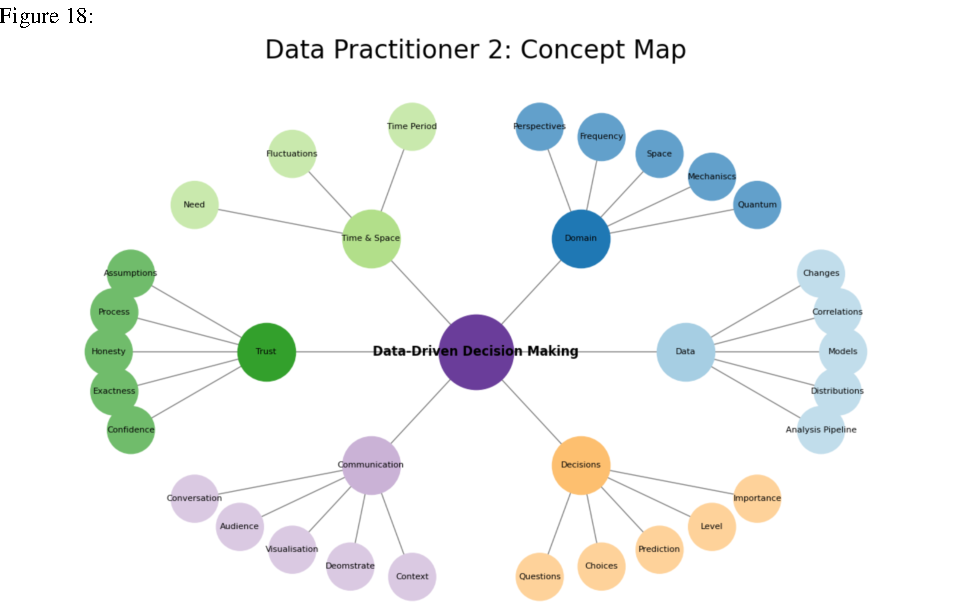
\includegraphics{210431461_CSC8639_Dissertation_files/figure-latex/unnamed-chunk-14-1.pdf}

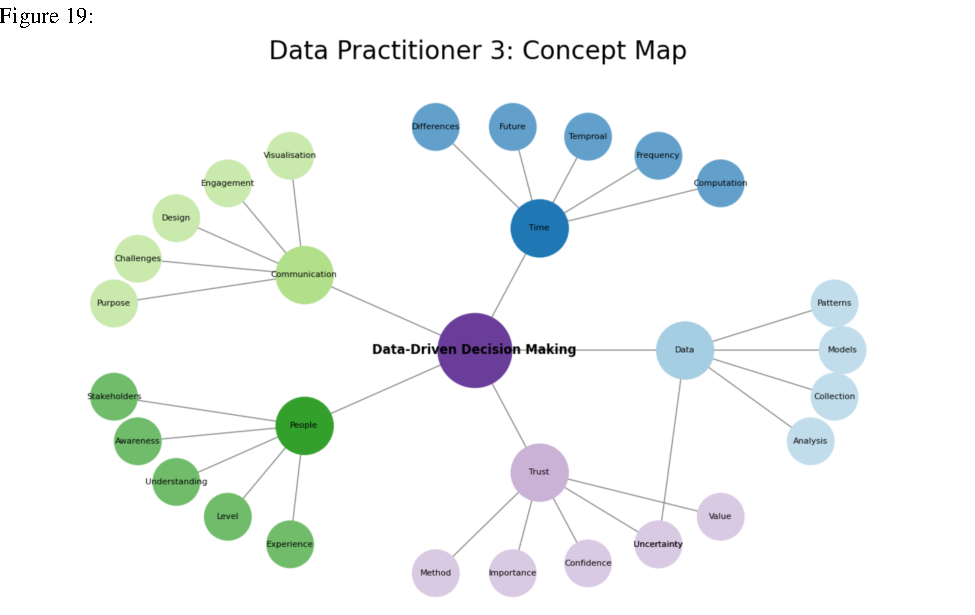
\includegraphics{210431461_CSC8639_Dissertation_files/figure-latex/unnamed-chunk-15-1.pdf}

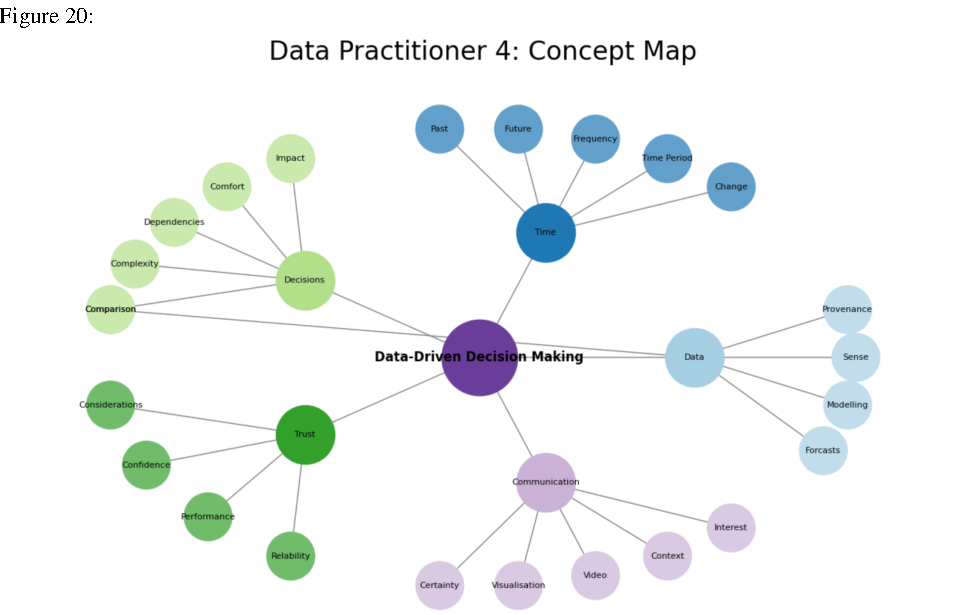
\includegraphics{210431461_CSC8639_Dissertation_files/figure-latex/unnamed-chunk-16-1.pdf}

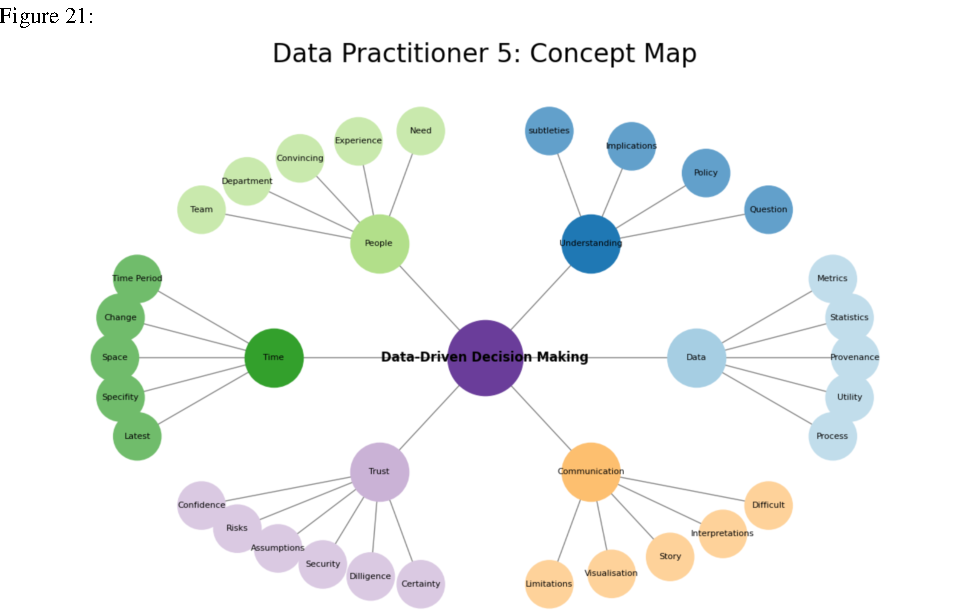
\includegraphics{210431461_CSC8639_Dissertation_files/figure-latex/unnamed-chunk-17-1.pdf}

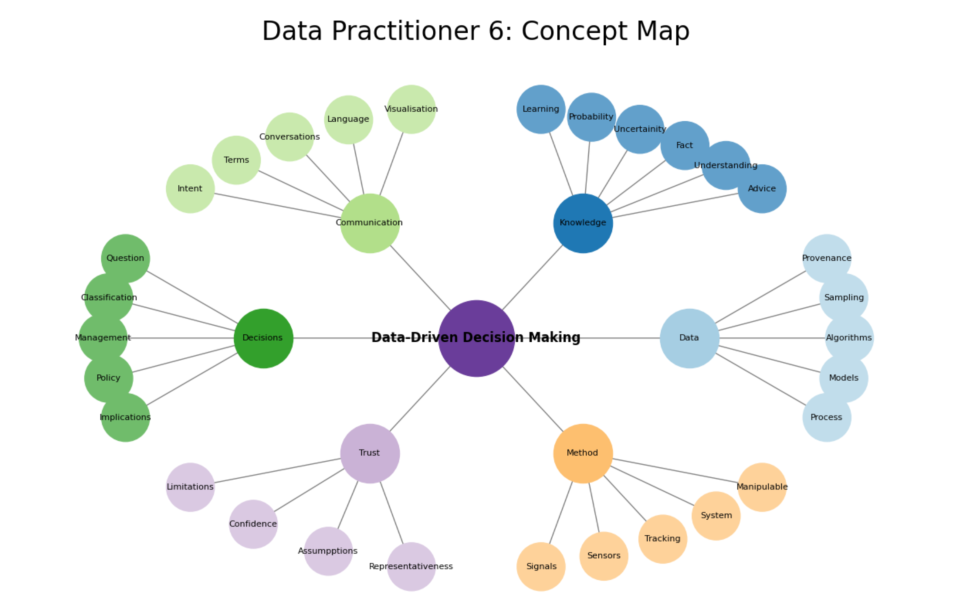
\includegraphics{210431461_CSC8639_Dissertation_files/figure-latex/unnamed-chunk-18-1.pdf}

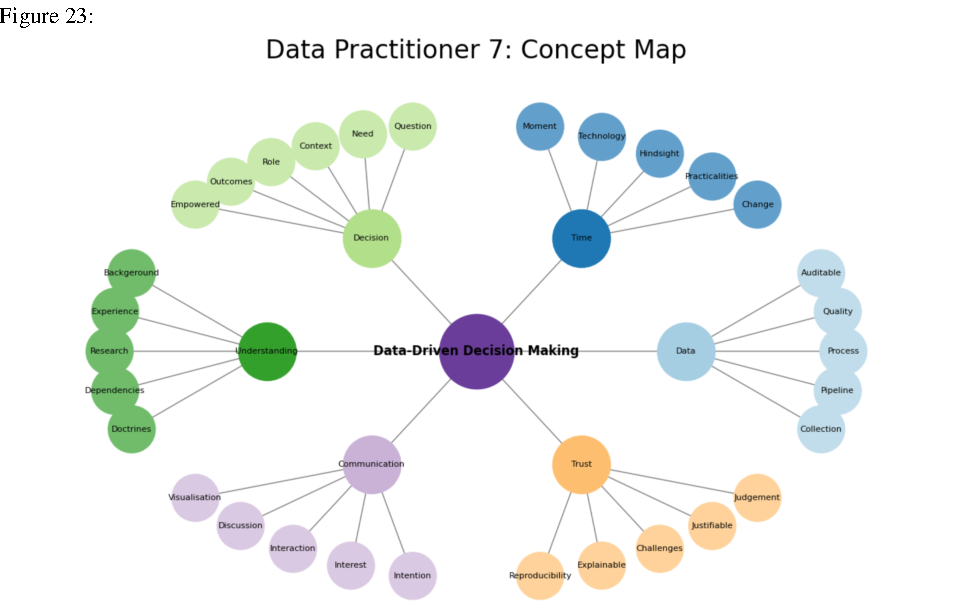
\includegraphics{210431461_CSC8639_Dissertation_files/figure-latex/unnamed-chunk-19-1.pdf}

\newpage

\hypertarget{annex-d-original-nine-synthetic-time-series}{%
\section{Annex D: Original Nine Synthetic Time
Series}\label{annex-d-original-nine-synthetic-time-series}}

\vspace{-0.4cm}

Each line plot in Figure 24 below visualises one of the nine original
synthetic time series from the Alan Turing Institute data set
\protect\hyperlink{ref-ATIChangePoint}{{[}45{]}}.

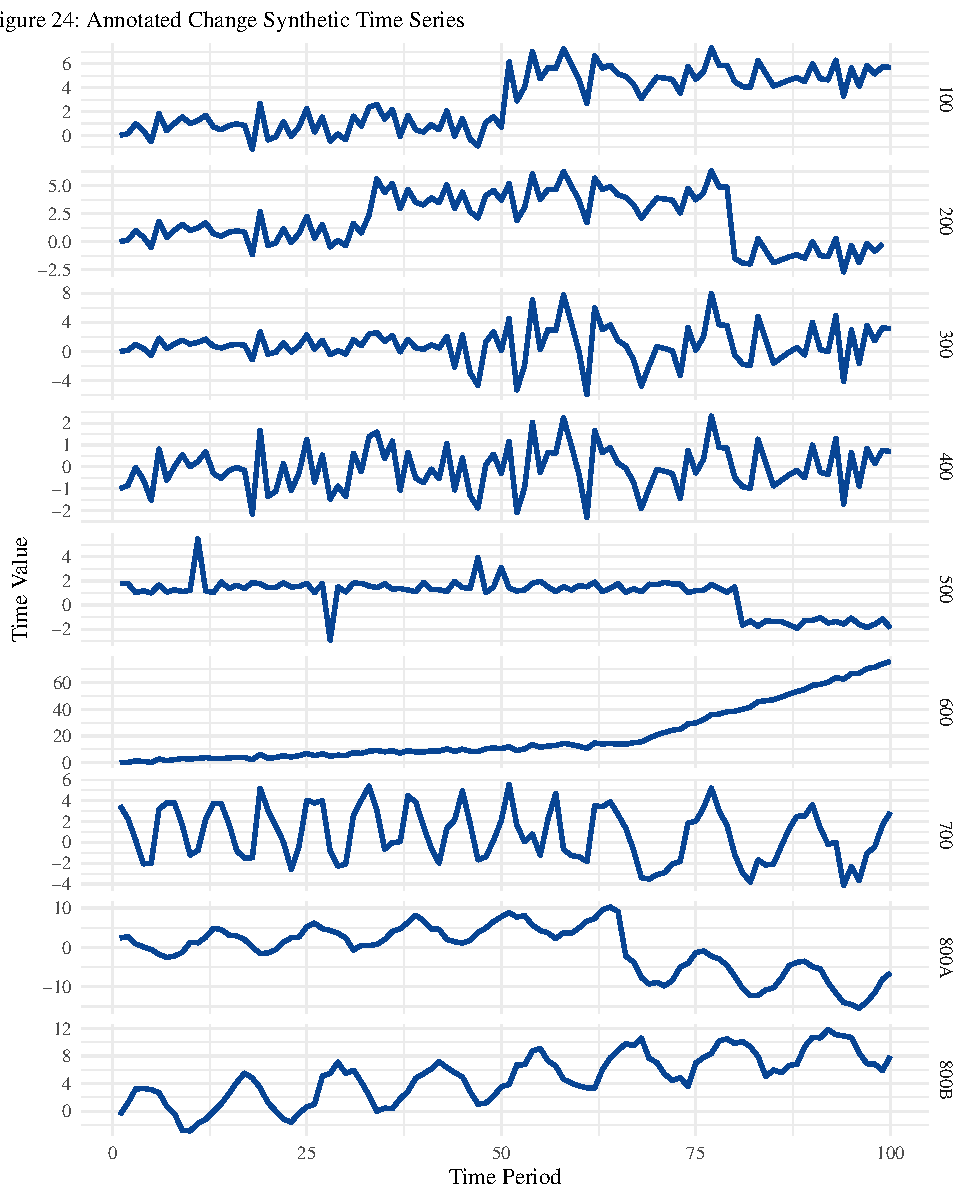
\includegraphics{210431461_CSC8639_Dissertation_files/figure-latex/unnamed-chunk-20-1.pdf}

\newpage

\hypertarget{annex-e-coefficient-of-variation-for-all-catch22-features}{%
\section{\texorpdfstring{Annex E: Coefficient of Variation for all
\texttt{Catch22}
Features}{Annex E: Coefficient of Variation for all Catch22 Features}}\label{annex-e-coefficient-of-variation-for-all-catch22-features}}

\vspace{-0.3cm}

Figure 25 visualises the absolute coefficient of variation values for
each \texttt{catch22} time series feature.

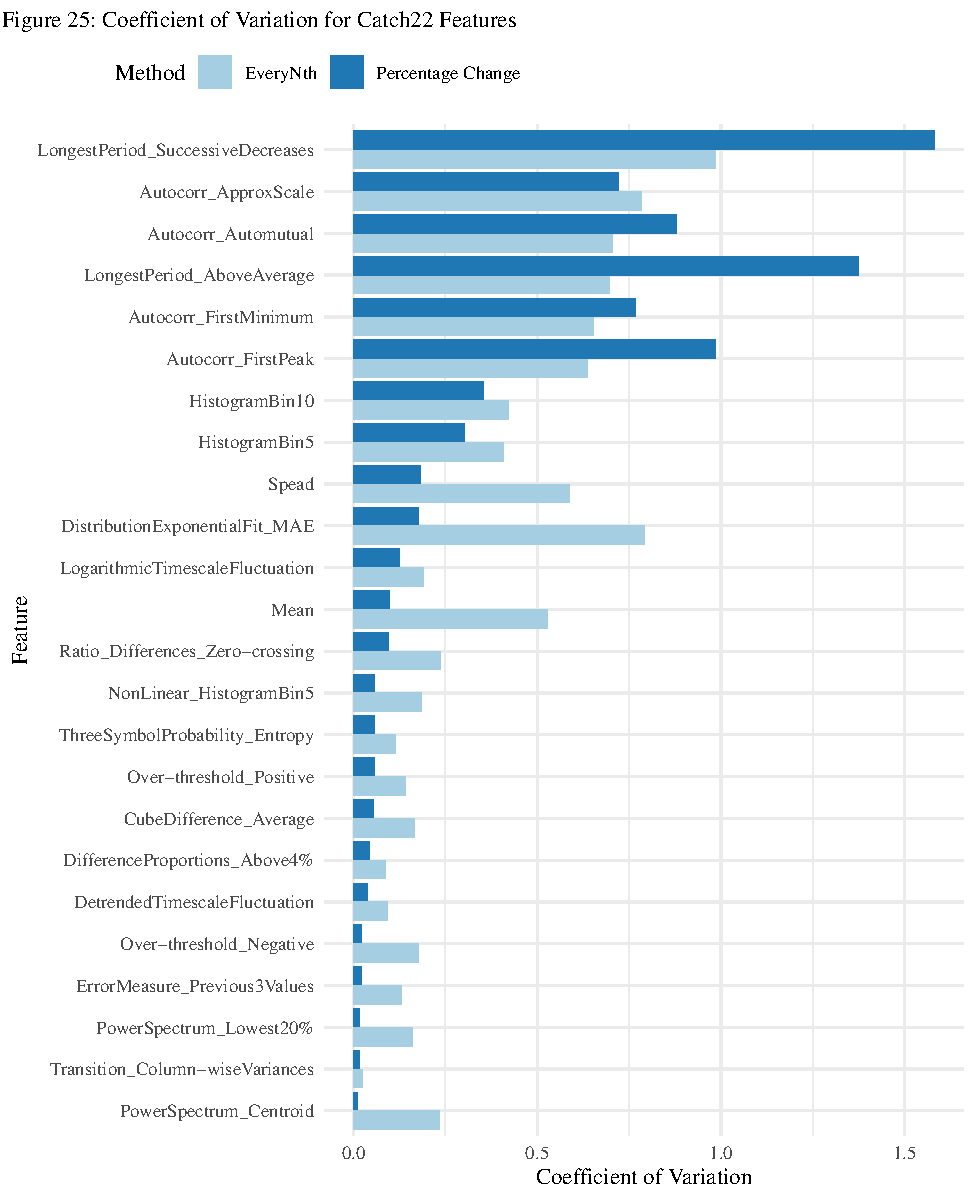
\includegraphics{210431461_CSC8639_Dissertation_files/figure-latex/unnamed-chunk-21-1.pdf}

\hypertarget{annex-f-the-statistical-properties-of-catch22-features}{%
\section{\texorpdfstring{Annex F: The Statistical Properties of
\texttt{Catch22}
Features}{Annex F: The Statistical Properties of Catch22 Features}}\label{annex-f-the-statistical-properties-of-catch22-features}}

\renewcommand{\arraystretch}{1.5}
\begin{table}[H]

\caption{\label{tab:unnamed-chunk-22}Catch22 Feature Overview [47]}
\centering
\begin{tabular}[t]{>{\raggedright\arraybackslash}p{0.7in}|>{\raggedright\arraybackslash}p{2.1in}|>{\raggedright\arraybackslash}p{2.1in}|>{\raggedright\arraybackslash}p{1in}}
\hline
Category & Original Feature Name & Other Feature Name & Description\\
\hline
Distribution shape & DN\_HistogramMode\_5 & HistogramBin5 & 5-bin histogram mode\\
\hline
Distribution shape & DN\_HistogramMode\_10 & HistogramBin10 & 10-bin histogram mode\\
\hline
Extreme event timing & DN\_OutlierInclude\_p\_001\_ mdrmd & Over-threshold\_ Positive & Positive outlier timing\\
\hline
Extreme event timing & DN\_OutlierInclude\_n\_001\_ mdrmd & Over-threshold\_ Negative & Negative outlier timing\\
\hline
Linear autocorrelation & CO\_f1ecac & Autocorr\_ApproxScale & First  crossing of the ACF\\
\hline
Linear autocorrelation & CO\_FirstMin\_ac & Autocorr\_FirstMinimum & First minimum of the ACF\\
\hline
Linear autocorrelation structure & SP\_Summaries\_welch\_rect\_ area\_5\_1 & PowerSpectrum\_Lowest20\% & Power in lowest 20\% frequencies\\
\hline
Linear autocorrelation & SP\_Summaries\_welch\_rect\_ centroid & PowerSpectrum\_Centroid & Centroid frequency\\
\hline
Linear autocorrelation & PD\_PeriodicityWang\_th001 & Autocorr\_FirstPeak & Wang's periodicity metric\\
\hline
Simple forcasting & FC\_LocalSimple\_mean3\_ stderr & ErrorMeasure\_Previous3Values & Error of 3-point rolling mean forecast\\
\hline
Incremental differences & FC\_LocalSimple\_mean1\_ tauresrat & Ratio\_Differences\_Zero-crossing & Change in autocorrelation timescale after incremental differencing\\
\hline
Incremental differences & MD\_hrv\_classic\_ pnn40 & DifferenceProportions\_Above4\% & Proportion of high incremental changes in the series\\
\hline
Symbolic & SB\_BinaryStats\_mean\_ longstretch1 & LongestPeriod\_AboveAverage & Longest stretch of above-mean values\\
\hline
Symbolic & SB\_BinaryStats\_diff\_ longstretch0 & LongestPeriod\_SuccessiveDecreases & Longest stretch of decreasing values\\
\hline
\end{tabular}
\end{table}

\begin{table}[H]

\caption{\label{tab:unnamed-chunk-23}Catch22 Feature Overview Continued [47]}
\centering
\begin{tabular}[t]{>{\raggedright\arraybackslash}p{0.7in}|>{\raggedright\arraybackslash}p{2.3in}|>{\raggedright\arraybackslash}p{2.1in}|>{\raggedright\arraybackslash}p{1in}}
\hline
Symbolic & SB\_MotifThree\_quantile\_hh & ThreeSymbolProbability\_Entropy & Entropy of successive pairs in symbolized series\\
\hline
Symbolic & SB\_TransitionMatrix\_3ac\_sumdiagcov & Transition\_Column-wiseVariances & Transition matrix column variance\\
\hline
Non-linear autocorrelation & CO\_HistogramAMI\_even\_2\_5 & NonLinear\_HistogramBin5 & Histogram-based automutual information (lag 2, 5 bins)\\
\hline
Non-linear autocorrelation & CO\_trev\_1\_num & CubeDifference\_Average & Time reversibility\\
\hline
Non-linear autocorrelation & IN\_AutoMutualInfoStats\_40\_ gaussian\_fmmi & Autocorr\_Automutual & First minimum of the AMI function\\
\hline
Self-affine scaling & SC\_FluctAnal\_2\_rsrangefit\_50\_1\_ logi\_prop\_r1 & LogarithmicTimescaleFluctuation & Rescaled range fluctuation analysis (low-scale scaling)\\
\hline
Self-affine scaling & SC\_FluctAnal\_2\_dfa\_50\_1\_2\_logi\_ prop\_r1 & DetrendedTimescaleFluctuation & Detrended fluctuation analysis (low-scale scaling)\\
\hline
Other & CO\_Embed2\_Dist\_tau\_d\_expfit\_ meandiff & DistributionExponentialFit\_MAE & Goodness of exponential fit to embedding distance distribution\\
\hline
Other & DN\_Mean & Mean & Mean\\
\hline
Other & DN\_Spread\_Std & Spread & Standard Deviation\\
\hline
\end{tabular}
\end{table}

It is interesting to note that the seven most sensitive \texttt{catch22}
features are in three categories: \texttt{symbolic},
\texttt{linear\ autocorrelation}, and \texttt{other}. Further
investigation to understand why would be beneficial.

\newpage

\hypertarget{annex-g-variation-of-catch22-features-across-time-series-types}{%
\section{\texorpdfstring{Annex G: Variation of \texttt{Catch22} Features
across Time Series
Types}{Annex G: Variation of Catch22 Features across Time Series Types}}\label{annex-g-variation-of-catch22-features-across-time-series-types}}

Figure 26 presents the feature with the highest absolute coefficient of
variation across the 900 time series (\texttt{LongestPeriod\_Decreases}
or \texttt{SB\_BinaryStats\_diff\_longstretch0}). This catch22 feature
\emph{``calculates the longest sequence of successive steps in the time
series that decrease''} \protect\hyperlink{ref-feature_book}{{[}48{]}}.
Initial visual analysis suggests that time series `100,' `300,' and
`500' are most affected by this feature.

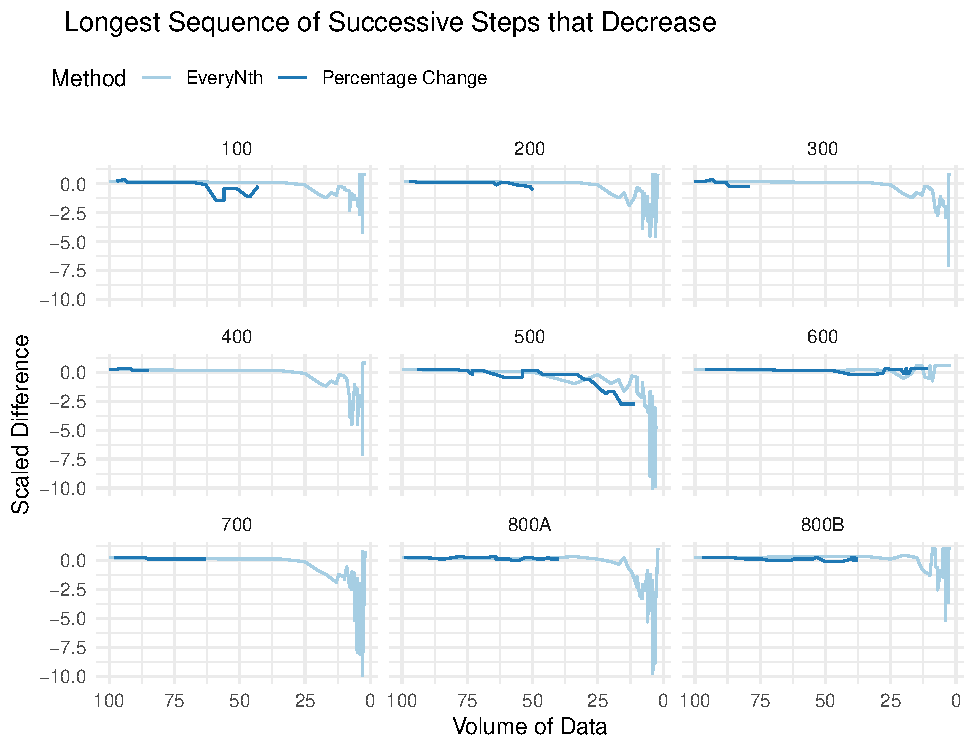
\includegraphics{210431461_CSC8639_Dissertation_files/figure-latex/LongestDecrease-1.pdf}

\newpage

Figure 27 presents the feature with the second highest absolute
coefficient of variation (\texttt{Autocorr\_FirstMinimum} or
\texttt{CO\_FirstMin\_ac}). This catch22 feature \emph{``computes the
first minimum of the autocorrelation function''}
\protect\hyperlink{ref-feature_book}{{[}48{]}}. Initial visual analysis
suggests that time series `100,' `200' and `500' are more affected by
this feature.

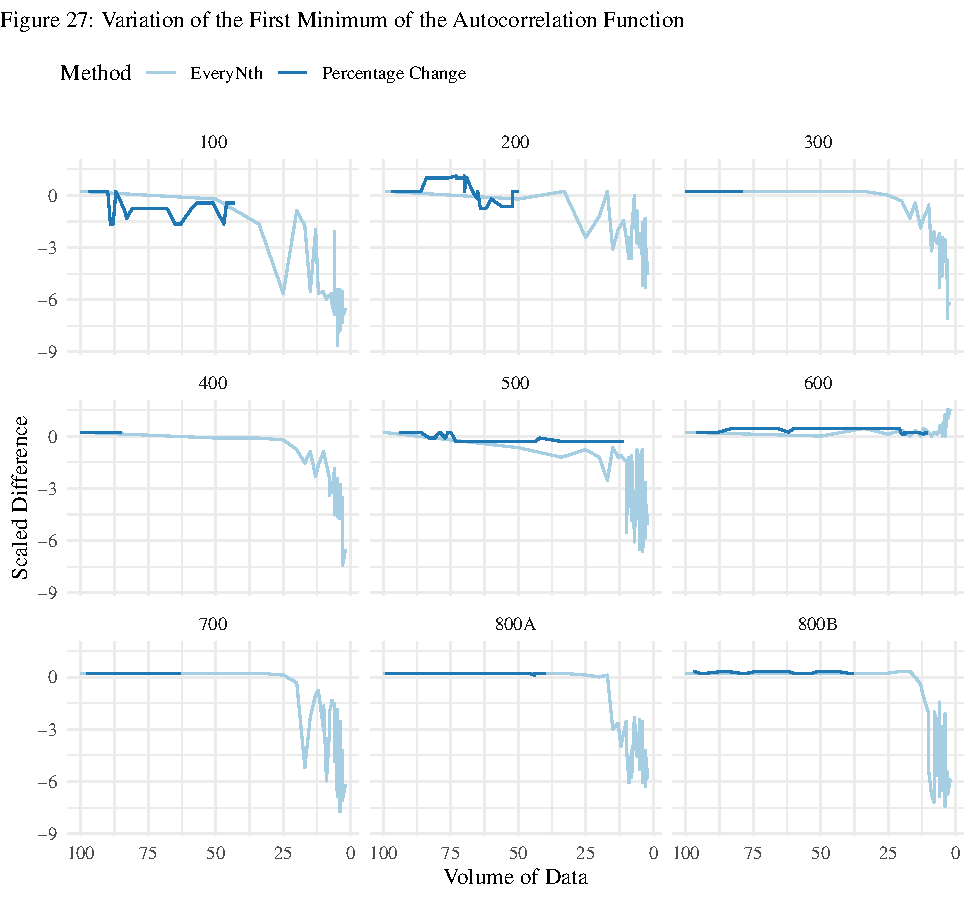
\includegraphics{210431461_CSC8639_Dissertation_files/figure-latex/FirstMinimum2-1.pdf}

\newpage

Figure 28 presents the feature with the third highest absolute
coefficient of variation (\texttt{Autocorr\_Automutual} or
\texttt{IN\_AutoMutualInfoStats\_40\_gaussian\_fmmi}). This catch22
feature outputs a measure of \emph{``autocorrelation in the time series,
as the minimum of the automutual information function''}
\protect\hyperlink{ref-feature_book}{{[}48{]}}. Initial visual analysis
suggests that time series `100,' `200,' `500,' and `600' are more
affected by this feature.

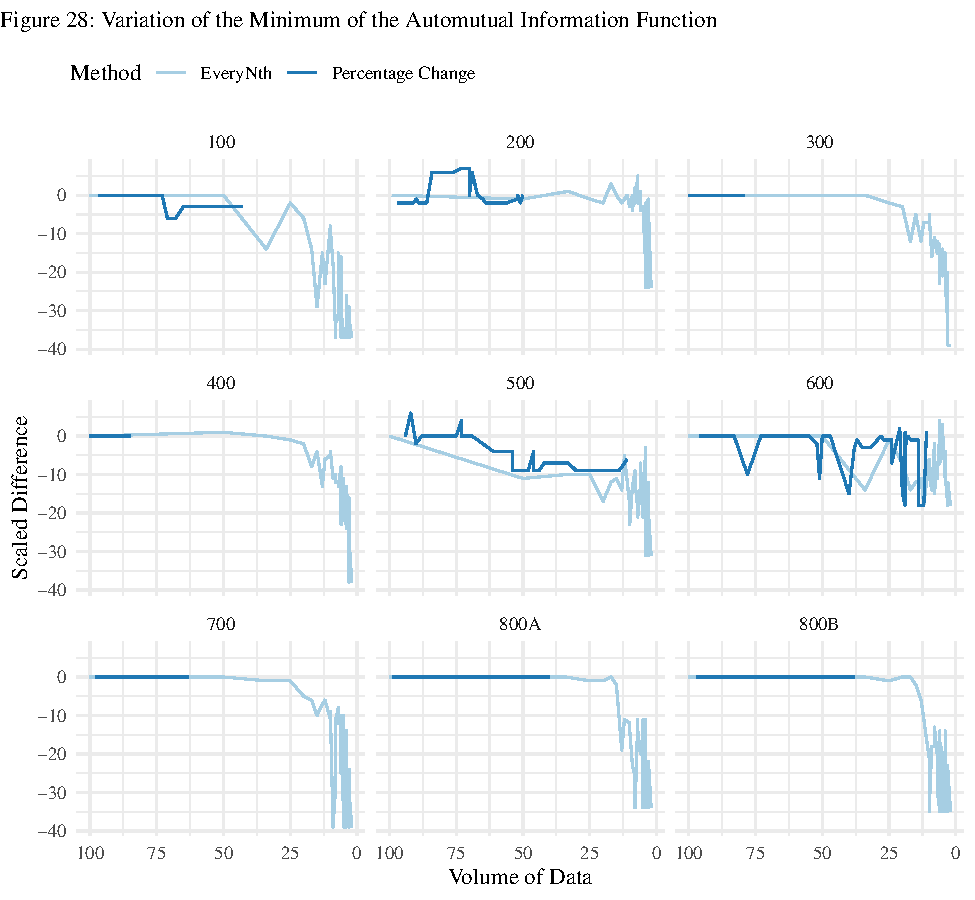
\includegraphics{210431461_CSC8639_Dissertation_files/figure-latex/AutoMutalFunction-1.pdf}

\newpage

Figure 29 presents the feature with the fourth highest absolute
coefficient of variation (\texttt{LongestPeriod\_AboveAverage} or
\texttt{SB\_BinaryStats\_mean\_longstretch1}). This catch22 feature
\emph{``calculates the longest successive period of above average
values''} \protect\hyperlink{ref-feature_book}{{[}48{]}}. Initial visual
analysis suggests that time series `200,' `500,' and `800B' are more
affected by this feature.

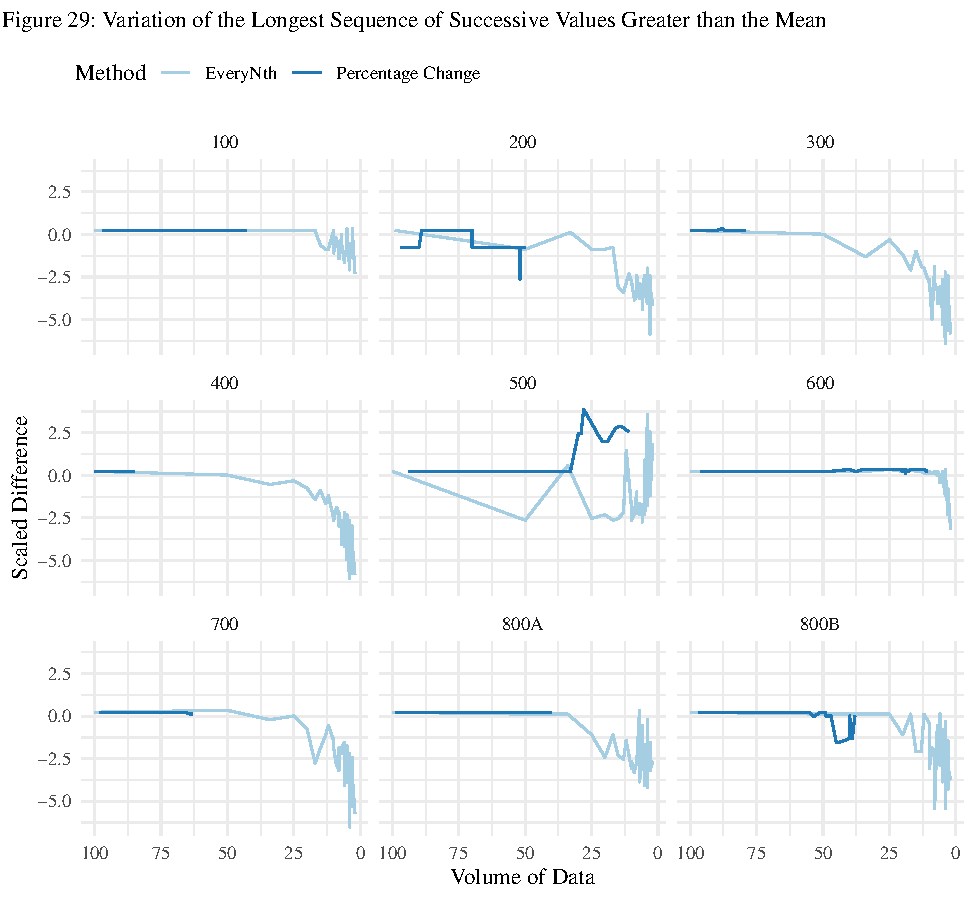
\includegraphics{210431461_CSC8639_Dissertation_files/figure-latex/LongestGreater-1.pdf}

\newpage

Figure 30 presents the feature with the fifth highest absolute
coefficient of variation (\texttt{Autocorr\_ApproxScale} or
\texttt{CO\_f1ecac}). This catch22 feature \emph{``computes the first
1/e crossing of the autocorrelation function of the time series''}
\protect\hyperlink{ref-feature_book}{{[}48{]}}. It is similar to the
first minimum of the autocorrelation function. Initial visual analysis
suggests that time series `100,' `200,' `500,' `800A' and `800B' are
more affected by this feature.

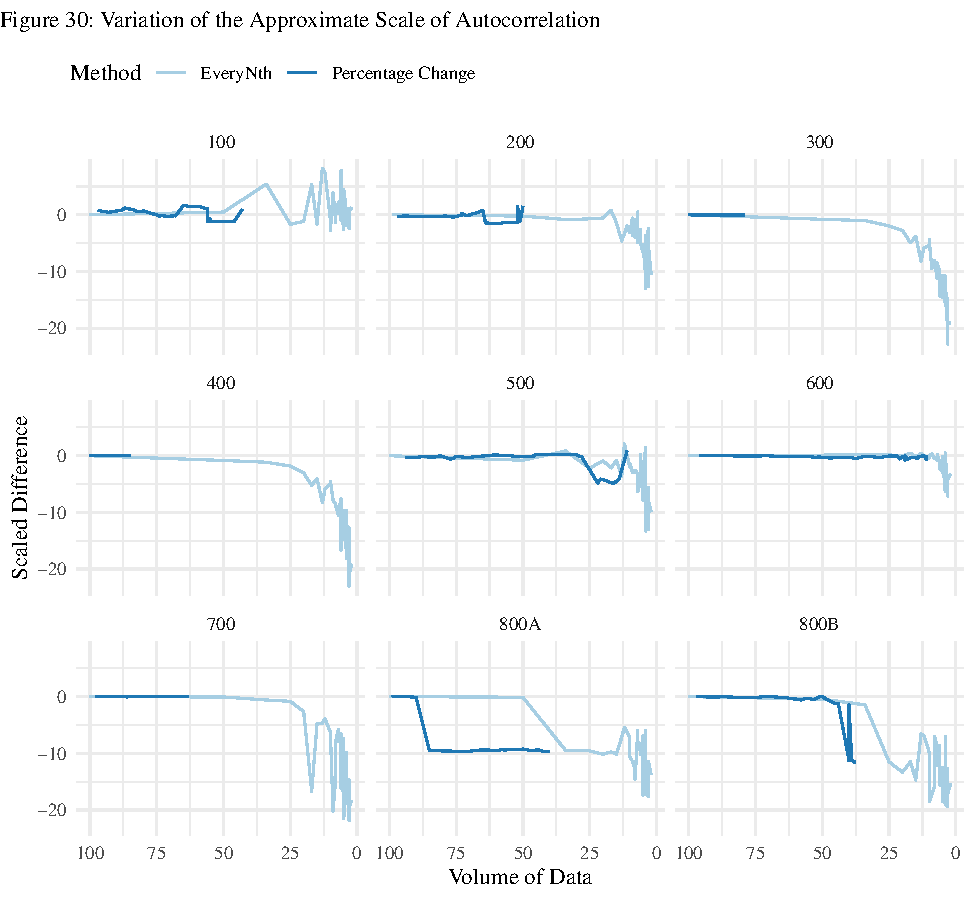
\includegraphics{210431461_CSC8639_Dissertation_files/figure-latex/ApproxScale-1.pdf}

\newpage

Figure 31 presents the feature with the sixth highest absolute
coefficient of variation (\texttt{Autocorr\_FirstPeak} or
\texttt{PD\_PeriodicityWang\_th0\_01}). This catch22 feature
\emph{``returns the first peak in the autocorrelation function
satisfying a set of conditions (after detrending the time series using a
single-knot cubic regression spline)''}
\protect\hyperlink{ref-feature_book}{{[}48{]}}. In general, the feature
returns higher values for slower time series oscillation. Initial visual
analysis suggests that time series `100,' `200' and `500' are more
affected by this feature.

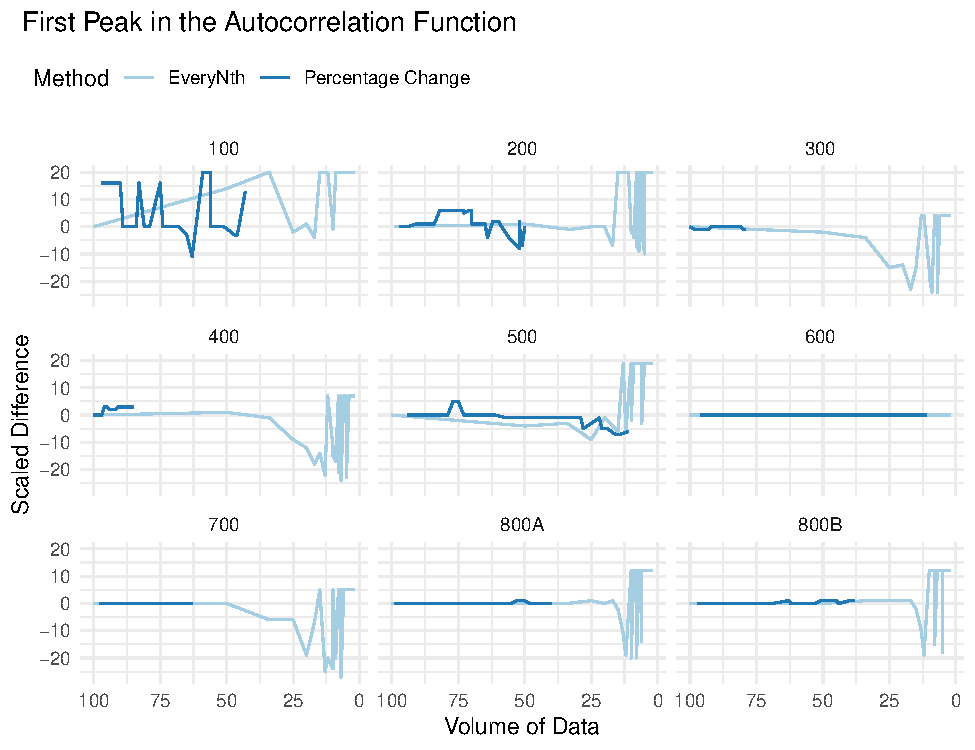
\includegraphics{210431461_CSC8639_Dissertation_files/figure-latex/FirstPeak-1.pdf}

\newpage

\hypertarget{annex-h-most-sensitive-catch22-features-for-each-time-series-type}{%
\section{\texorpdfstring{Annex H: Most Sensitive \texttt{Catch22}
Features for each Time Series
Type}{Annex H: Most Sensitive Catch22 Features for each Time Series Type}}\label{annex-h-most-sensitive-catch22-features-for-each-time-series-type}}

Figure 32 visualises the six most sensitive features for time series
100. Initial visual analysis suggests that
\texttt{Autocorr\_FirstMinimum}, \texttt{Autocorr\_FirstPeak} and
\texttt{LongestPeriod\_Decreases} may best indicate the impact of
downsampling for this time series.

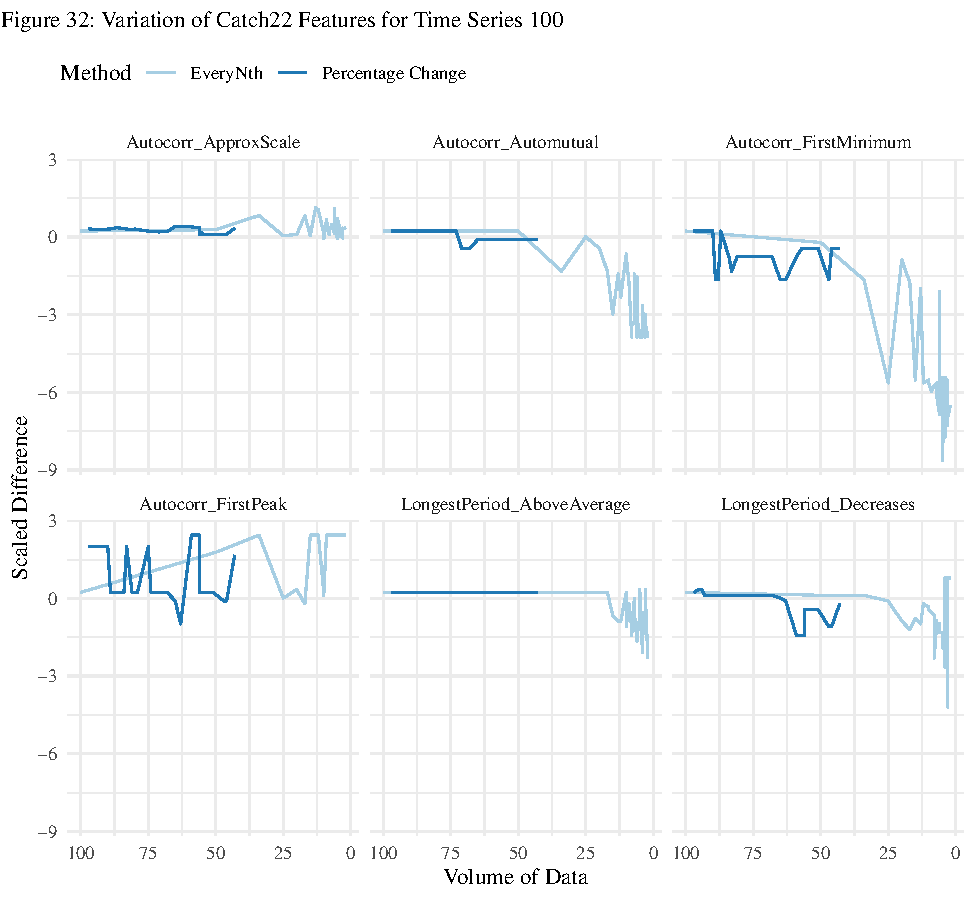
\includegraphics{210431461_CSC8639_Dissertation_files/figure-latex/Catch22Variation100-1.pdf}

\newpage

Figure 33 visualises the six most sensitive features for time series
200. \texttt{Autocorr\_Automutual}, \texttt{Autocorr\_FirstMinimum},
\texttt{Autocorr\_FirstPeak} and \texttt{LongestPeriod\_AboveAverage}
may best indicate the impact of downsampling for this time series.

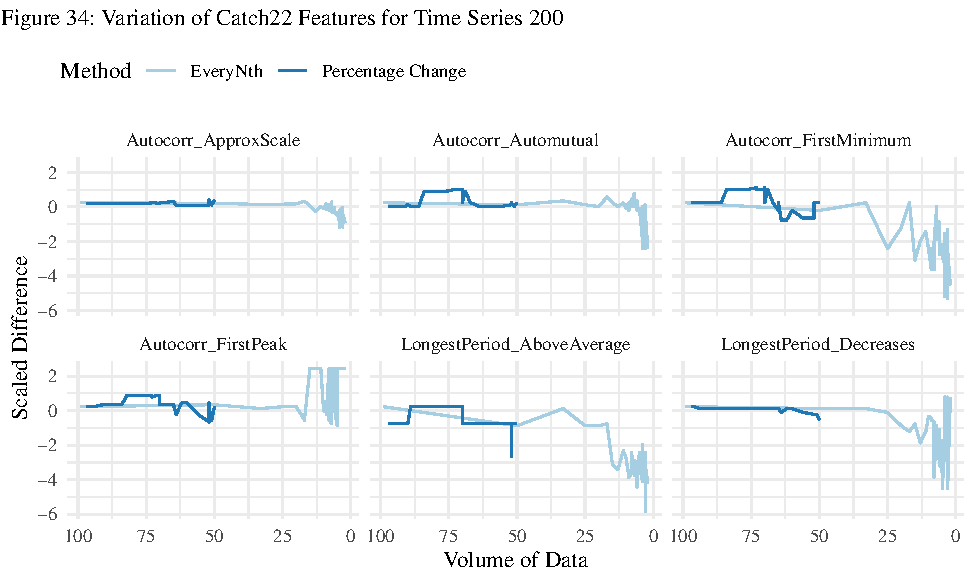
\includegraphics{210431461_CSC8639_Dissertation_files/figure-latex/Catch22Variation200-1.pdf}

Figure 34 visualises the six most sensitive features for time series
300. \texttt{Autocorr\_FirstPeak}, \texttt{LongestPeriod\_AboveAverage}
and \texttt{LongestPeriod\_Decreases} may best indicate the impact of
downsampling for this time series.

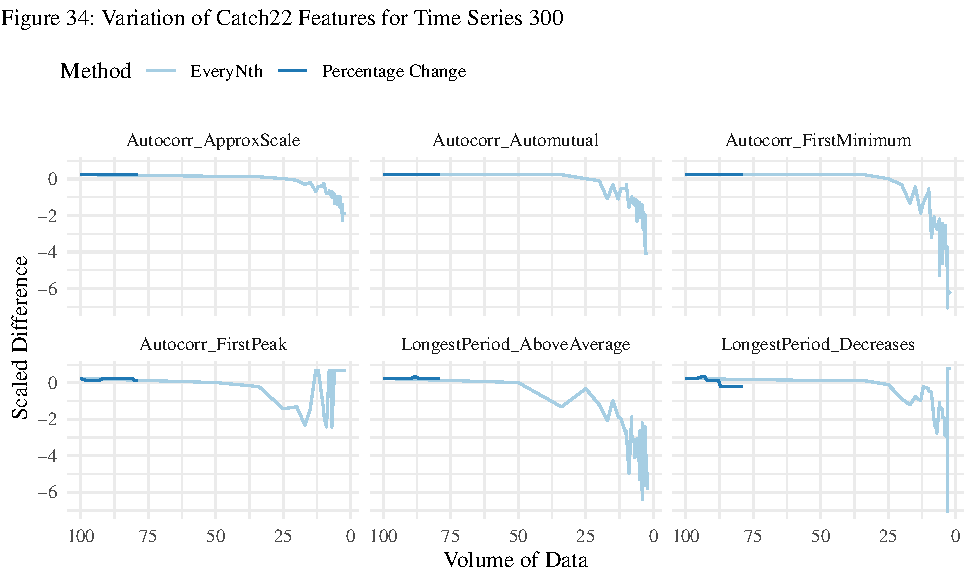
\includegraphics{210431461_CSC8639_Dissertation_files/figure-latex/Catch22Variation300-1.pdf}

Figure 35 visualises the six most sensitive features for time series
400. \texttt{Autocorr\_FirstPeak} and \texttt{LongestPeriod\_Decreases}
may best indicate the impact of downsampling for this time series.

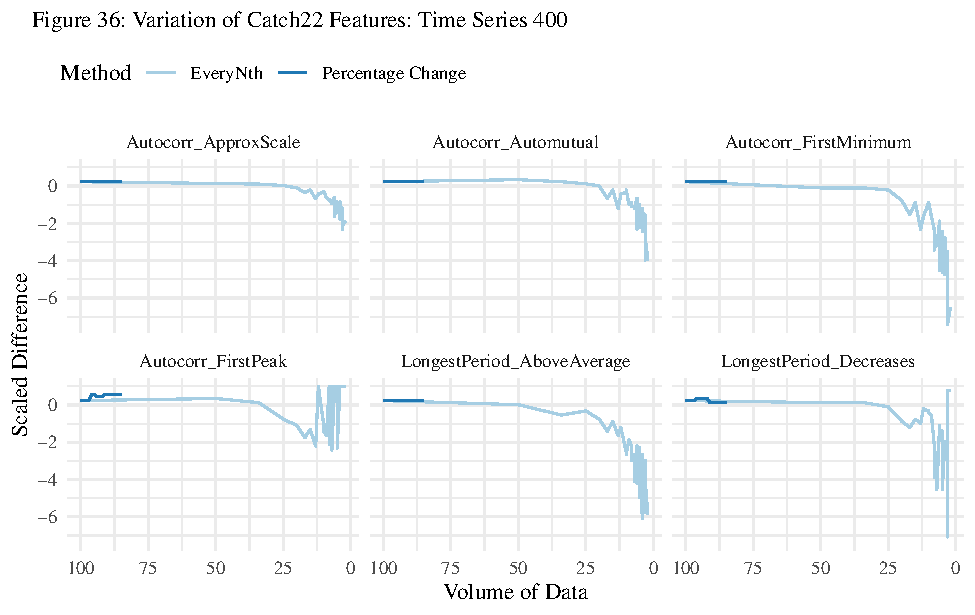
\includegraphics{210431461_CSC8639_Dissertation_files/figure-latex/Catch22Variation400-1.pdf}

Figure 36 visualises the six most sensitive features for time series
500. \texttt{Autocorr\_Automutual}, \texttt{Autocorr\_FirstMinimum}, and
\texttt{Autocorr\_FirstPeak} may best indicate the impact of
downsampling for this time series.

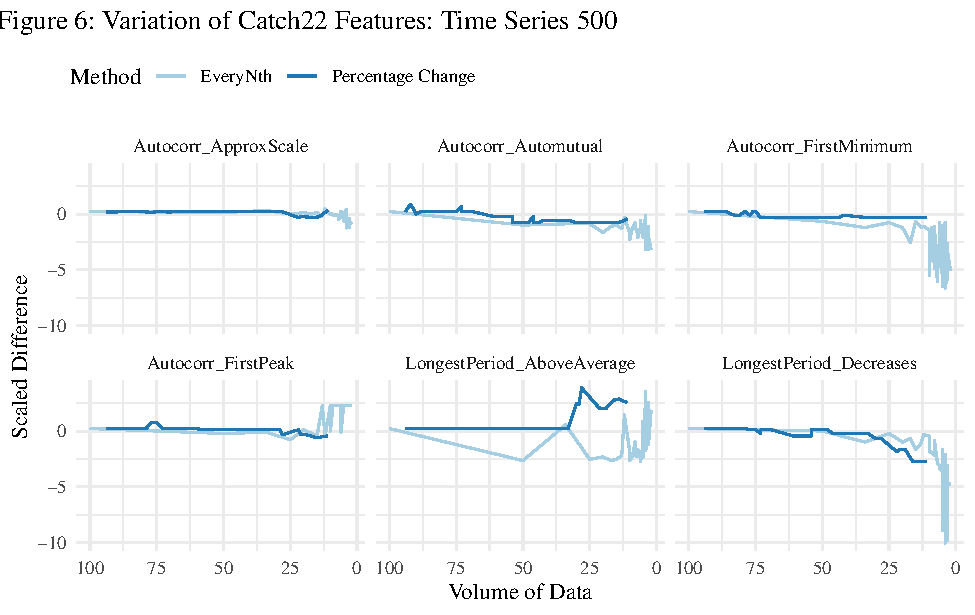
\includegraphics{210431461_CSC8639_Dissertation_files/figure-latex/Catch22Variation500-1.pdf}

\newpage

Figure 37 visualises the six most sensitive features for time series
600. \texttt{Autocorr\_Automutual} and \texttt{Autocorr\_FirstMinimum}
may best indicate the impact of downsampling for this time series.

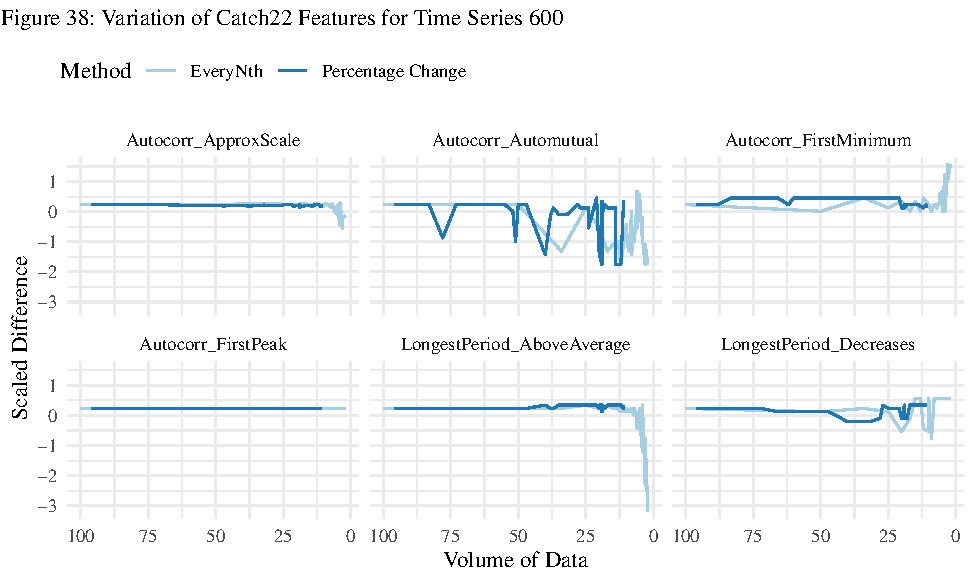
\includegraphics{210431461_CSC8639_Dissertation_files/figure-latex/Catch22Variation600-1.pdf}

Figure 38 visualises the six most sensitive features for time series
700. \texttt{LongestPeriod\_AboveAverage} and
\texttt{LongestPeriod\_Decreases} may best indicate the impact of
downsampling for this time series.

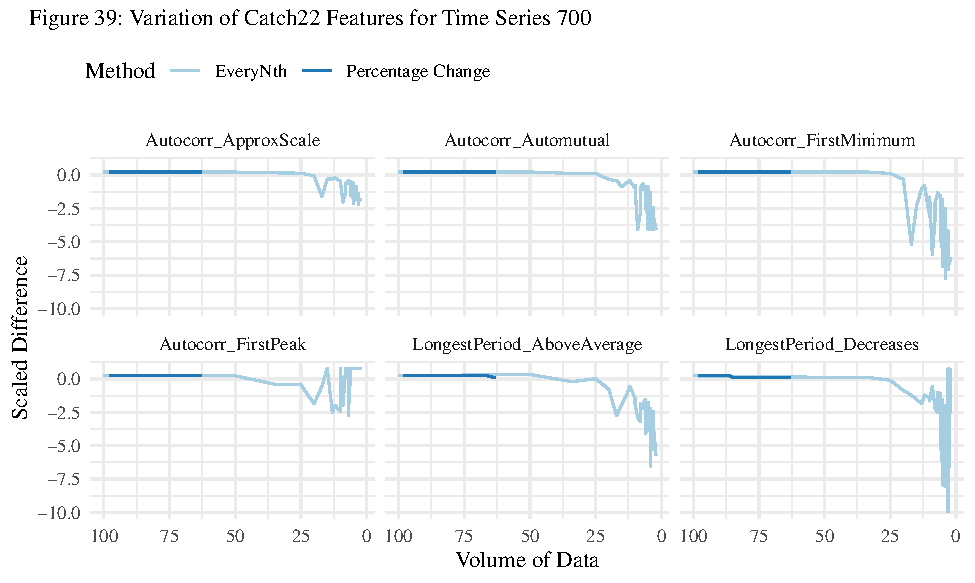
\includegraphics{210431461_CSC8639_Dissertation_files/figure-latex/Catch22Variation700-1.pdf}

\newpage

Figure 39 visualises the six most sensitive features for time series
800A. \texttt{Autocorr\_ApproxScale} and
\texttt{LongestPeriod\_Decreases} may best indicate the impact of
downsampling for this time series.

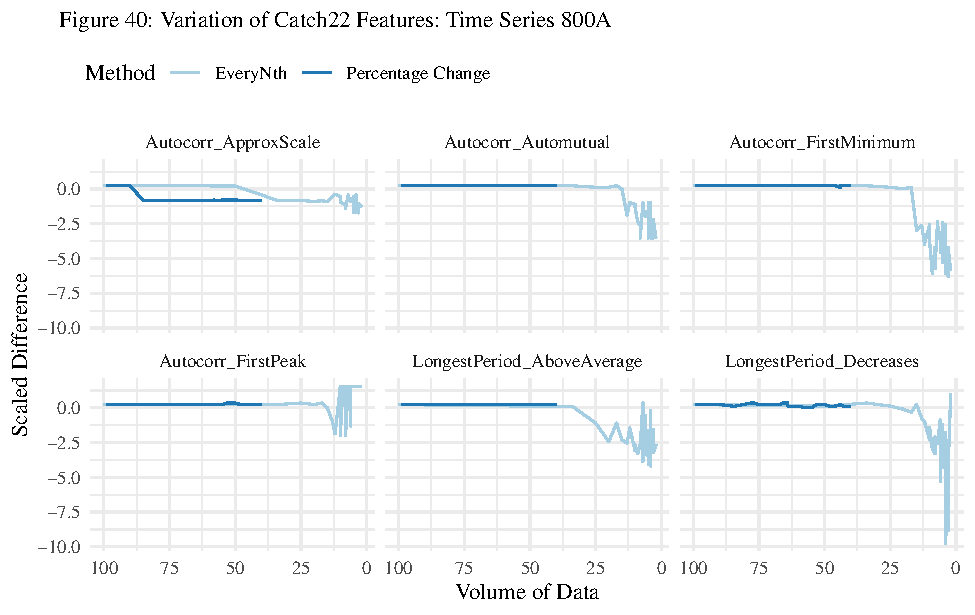
\includegraphics{210431461_CSC8639_Dissertation_files/figure-latex/Catch22Variation800A-1.pdf}

Figure 40 visualises the six most sensitive features for time series
800A. \texttt{Autocorr\_ApproxScale}, \texttt{Autocorr\_FirstMinimum},
\texttt{LongestPeriod\_AboveAverage} and
\texttt{LongestPeriod\_Decreses} may best indicate the impact of
downsampling for this time series.

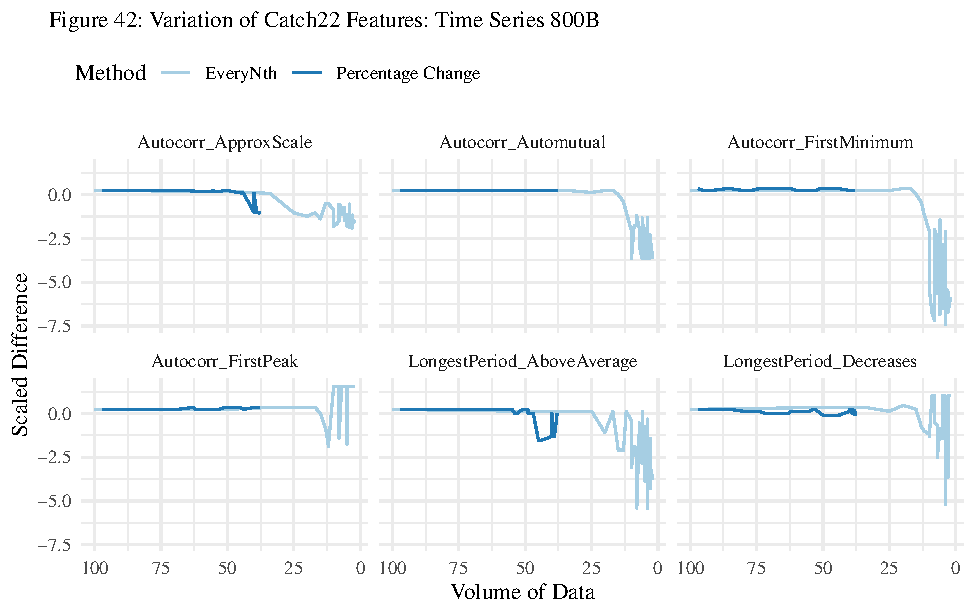
\includegraphics{210431461_CSC8639_Dissertation_files/figure-latex/Catch22Variation800B-1.pdf}

\newpage

\hypertarget{references}{%
\section*{REFERENCES}\label{references}}
\addcontentsline{toc}{section}{REFERENCES}

\hypertarget{refs}{}
\begin{CSLReferences}{0}{0}
\leavevmode\vadjust pre{\hypertarget{ref-data2017}{}}%
\CSLLeftMargin{{[}1{]} }
\CSLRightInline{Cabinet Office and Government Digital Service,
{``Government transformation strategy: Better use of data.''} HM
Government;
\url{https://www.gov.uk/government/publications/government-transformation-strategy-2017-to-2020/government-transformation-strategy-better-use-of-data},
Accessed: 23, 07, 2017.}

\leavevmode\vadjust pre{\hypertarget{ref-data2020}{}}%
\CSLLeftMargin{{[}2{]} }
\CSLRightInline{Department for Digital, Culture, Media \& Sport and
Department for Science, Innovation \& Technology, {``National data
strategy.''} HM Government;
\url{https://www.gov.uk/government/publications/uk-national-data-strategy/national-data-strategy},
Accessed: 23, 07, 2020.}

\leavevmode\vadjust pre{\hypertarget{ref-data2021}{}}%
\CSLLeftMargin{{[}3{]} }
\CSLRightInline{M. of Defence, {``Data strategy for defence,''}
\emph{GOV.UK}. HM Government;
\url{https://www.gov.uk/government/publications/data-strategy-for-defence/data-strategy-for-defence},
Accessed: 23, 07, 2021.}

\leavevmode\vadjust pre{\hypertarget{ref-data2022}{}}%
\CSLLeftMargin{{[}4{]} }
\CSLRightInline{Central Digital \& Data Office, {``Transforming for a
digital future: 2022 to 2025 roadmap for digital and data.''} HM
Government;
\url{https://www.gov.uk/government/publications/roadmap-for-digital-and-data-2022-to-2025/transforming-for-a-digital-future-2022-to-2025-roadmap-for-digital-and-data},
Accessed: 23, 07, 2022.}

\leavevmode\vadjust pre{\hypertarget{ref-trust}{}}%
\CSLLeftMargin{{[}5{]} }
\CSLRightInline{Centre for Data Ethics \& Innovation, {``Addressing
trust in public sector data use.''}
\url{https://www.gov.uk/government/publications/cdei-publishes-its-first-report-on-public-sector-data-sharing/addressing-trust-in-public-sector-data-use\#introduction--context},
Accessed: 23, 07.}

\leavevmode\vadjust pre{\hypertarget{ref-datapoint}{}}%
\CSLLeftMargin{{[}6{]} }
\CSLRightInline{J. Donckt, J. Donckt, M. Rademaker, and S. Hoecke,
{``Data point selection for line chart visualization: Methodological
assessment and evidence-based guidelines.''} 2023. doi:
\href{https://doi.org/10.48550/arXiv.2304.00900}{10.48550/arXiv.2304.00900}.}

\leavevmode\vadjust pre{\hypertarget{ref-MinMaxLTTB}{}}%
\CSLLeftMargin{{[}7{]} }
\CSLRightInline{J. Donckt, J. Donckt, M. Rademaker, and S. Hoecke,
{``MinMaxLTTB: Leveraging MinMax-preselection to scale LTTB.''}
\url{https://arxiv.org/abs/2305.00332}, Accessed: 23, 07, 2023.}

\leavevmode\vadjust pre{\hypertarget{ref-pathway}{}}%
\CSLLeftMargin{{[}8{]} }
\CSLRightInline{Government Analysis Function, {``Types of data in
government learning pathway.''}
\url{https://analysisfunction.civilservice.gov.uk/learning-development/learning-pathways/types-of-data-in-government-learning-pathway/},
Accessed: 23, 07, 2022.}

\leavevmode\vadjust pre{\hypertarget{ref-onstool}{}}%
\CSLLeftMargin{{[}9{]} }
\CSLRightInline{Office for National Statistics, {``Time series
explorer.''}
\url{https://www.ons.gov.uk/timeseriestool?query=\&topic=\&updated=\&fromDateDay=\&fromDateMonth=\&fromDateYear=\&toDateDay=\&toDateMonth=\&toDateYear=\&size=50},
Accessed: 23, 07, Unknown.}

\leavevmode\vadjust pre{\hypertarget{ref-TVStore}{}}%
\CSLLeftMargin{{[}10{]} }
\CSLRightInline{Y. An, Y. Su, Y. Zhu, and J. Wang, {``TVStore:
Automatically bounding time series storage via time-varying
compression,''} in \emph{Proceedings of the 20th USENIX conference on
file and storage technologies}, in USENIX conference on file and STorage
technologies. Santa Clara, CA, USA: USENIX Association, 2022, pp.
83--99.}

\leavevmode\vadjust pre{\hypertarget{ref-Sveinn}{}}%
\CSLLeftMargin{{[}11{]} }
\CSLRightInline{S. Steinarsson, {``Downsampling time series for visual
representation.''} University of Iceland, Faculty of Industrial
Engineering, Mechanical Engineering; Computer Science, School of
Engineering; Natural Sciences, University of Iceland, Reykjavik,
Iceland, 2013.}

\leavevmode\vadjust pre{\hypertarget{ref-Shift}{}}%
\CSLLeftMargin{{[}12{]} }
\CSLRightInline{The Shift Project, {``Implementing digital
sufficiency.''}
\url{https://theshiftproject.org/wp-content/uploads/2021/07/TSP_DigitalSufficiency2020_Summary_corrige.pdf},
Accessed: 23, 07, 2020.}

\leavevmode\vadjust pre{\hypertarget{ref-downsampling}{}}%
\CSLLeftMargin{{[}13{]} }
\CSLRightInline{W. Aigner, S. Miksch, W. Muller, H. Schumann, and C.
Tominski, {``Visual methods for analyzing time-oriented data,''}
\emph{IEEE Transactions on Visualization and Computer Graphics}, vol.
14, no. 1, pp. 47--60, 2008, doi:
\href{https://doi.org/10.1109/TVCG.2007.70415}{10.1109/TVCG.2007.70415}.}

\leavevmode\vadjust pre{\hypertarget{ref-sampling}{}}%
\CSLLeftMargin{{[}14{]} }
\CSLRightInline{B. C. Kwon, J. Verma, P. J. Haas, and C. Demiralp,
{``Sampling for scalable visual analytics,''} \emph{IEEE Computer
Graphics and Applications}, vol. 37, no. 1, pp. 100--108, 2017, doi:
\href{https://doi.org/10.1109/MCG.2017.6}{10.1109/MCG.2017.6}.}

\leavevmode\vadjust pre{\hypertarget{ref-CISCO}{}}%
\CSLLeftMargin{{[}15{]} }
\CSLRightInline{B. Bechtold, {``Beyond the barrel: How data and
analytics will become the new currency in oil and gas.''}
/url{https://gblogs.cisco.com/ca/2018/06/07/beyond-the-barrel-how-data-and-analytics-will-become-the-new-currency-in-oil-and-gas/},
Accessed: 16, 08, 2018.}

\leavevmode\vadjust pre{\hypertarget{ref-challenger}{}}%
\CSLLeftMargin{{[}16{]} }
\CSLRightInline{D. Vaughan, \emph{The challenger launch decision: Risky
technology, culture, and deviance at NASA}. Chicago; London: The
University of Chicago Press, 1996.}

\leavevmode\vadjust pre{\hypertarget{ref-imputeTS_R}{}}%
\CSLLeftMargin{{[}17{]} }
\CSLRightInline{S. Moritz and T. Bartiz-Beielstein, {``imputeTS: Time
series missing value imputation in r,''} vol. 9.1.
\url{https://github.com/SteffenMoritz/imputeTS}; R Journal, Accessed:
23, 07, 2017. doi:
\href{https://doi.org/10.32614/RJ-2017-009}{10.32614/RJ-2017-009}.}

\leavevmode\vadjust pre{\hypertarget{ref-catch22_R}{}}%
\CSLLeftMargin{{[}18{]} }
\CSLRightInline{C. H. Lubba, B. Fulcher, T. Henderspn, B. Harris, O. r.
TL, and O. Cliff, {``catch22: CAnonical time-series CHaracteristics.''}
\url{https://github.com/DynamicsAndNeuralSystems/catch22}; R Journal,
Accessed: 23, 07, 2022. doi:
\href{https://doi.org/10.5281/zenodo.6673597}{10.5281/zenodo.6673597}.}

\leavevmode\vadjust pre{\hypertarget{ref-political_transparency}{}}%
\CSLLeftMargin{{[}19{]} }
\CSLRightInline{K. E. Levy and D. M. Johns, {``When open data is a
trojan horse: The weaponization of transparency in science and
governance,''} \emph{Big Data \& Society}, vol. 3, no. 1, 2016, doi:
\href{https://doi.org/10.1177/2053951715621568}{10.1177/2053951715621568}.}

\leavevmode\vadjust pre{\hypertarget{ref-social_transparency}{}}%
\CSLLeftMargin{{[}20{]} }
\CSLRightInline{J. Bates, H. Kennedy, I. Medina Perea, S. Oman, and L.
Pinney, {``Socially meaningful transparency in data-based systems:
Reflections and proposals from practice,''} \emph{Journal of
Documentation}, vol. ahead--of--print, 2023, doi:
\href{https://doi.org/10.1108/JD-01-2023-0006}{10.1108/JD-01-2023-0006}.}

\leavevmode\vadjust pre{\hypertarget{ref-transparency_lack}{}}%
\CSLLeftMargin{{[}21{]} }
\CSLRightInline{M. Ananny and K. Crawford, {``Seeing without knowing:
Limitations of the transparency ideal and its application to algorithmic
accountability,''} \emph{New Media \& Society}, vol. 20, no. 3, pp.
973--989, 2018, doi:
\href{https://doi.org/10.1177/1461444816676645}{10.1177/1461444816676645}.}

\leavevmode\vadjust pre{\hypertarget{ref-transparency_obfuscation}{}}%
\CSLLeftMargin{{[}22{]} }
\CSLRightInline{N. A. Draper and J. Turow, {``The corporate cultivation
of digital resignation,''} \emph{New Media \& Society}, vol. 21, no. 8,
pp. 1824--1839, 2019, doi:
\href{https://doi.org/10.1177/1461444819833331}{10.1177/1461444819833331}.}

\leavevmode\vadjust pre{\hypertarget{ref-transparency_fallacy}{}}%
\CSLLeftMargin{{[}23{]} }
\CSLRightInline{J. A. Obar, {``Sunlight alone is not a disinfectant:
Consent and the futility of opening big data black boxes (without
assistance),''} \emph{Big Data \& Society}, vol. 7, no. 1, 2020, doi:
\href{https://doi.org/10.1177/2053951720935615}{10.1177/2053951720935615}.}

\leavevmode\vadjust pre{\hypertarget{ref-timenotes}{}}%
\CSLLeftMargin{{[}24{]} }
\CSLRightInline{J. Walker, R. Borgo, and MW. Jones, {``Timeaddresss: A
study on effective chart visualization and interaction techniques for
time-series data,''} \emph{IEEE Transactions on Visualization and
Computer Graphics}, vol. 22, 2016, doi:
\href{https://doi.org/10.1109/TVCG.2015.2467751}{10.1109/TVCG.2015.2467751}.}

\leavevmode\vadjust pre{\hypertarget{ref-timetuner}{}}%
\CSLLeftMargin{{[}25{]} }
\CSLRightInline{J. Hao, Q. Shi, Y. Ye, and W. Zeng, {``TimeTuner:
Diagnosing time representations for time-series forecasting with
counterfactual explanations.''} 2023. doi:
\href{https://doi.org/10.48550/arXiv.2307.09916}{10.48550/arXiv.2307.09916}.}

\leavevmode\vadjust pre{\hypertarget{ref-plotly}{}}%
\CSLLeftMargin{{[}26{]} }
\CSLRightInline{J. Donckt, J. Donckt, E. Deprost, and S. Hoecke,
{``Plotly-resampler: Effective visual analytics for large time
series,''} \emph{IEEE Visualization and Visual Analytics}, 2022, doi:
\href{https://doi.org/10.1109/VIS54862.2022.00013}{10.1109/VIS54862.2022.00013}.}

\leavevmode\vadjust pre{\hypertarget{ref-imputeTS}{}}%
\CSLLeftMargin{{[}27{]} }
\CSLRightInline{S. Moritz and T. Bartiz-Beielstein, {``imputeTS: Time
series missing value imputation in r.''}
\url{https://cran.r-project.org/web/packages/imputeTS/vignettes/imputeTS-Time-Series-Missing-Value-Imputation-in-R.pdf};
R Journal, Accessed: 23, 07, 2017.}

\leavevmode\vadjust pre{\hypertarget{ref-missingdata}{}}%
\CSLLeftMargin{{[}28{]} }
\CSLRightInline{S. van Buuren, \emph{Flexible imputation of missing
data}. Accessed: 16, 08: /url{https://stefvanbuuren.name/fimd/};
Chapman; Hall, CRC Press, 2018.}

\leavevmode\vadjust pre{\hypertarget{ref-storage}{}}%
\CSLLeftMargin{{[}29{]} }
\CSLRightInline{A. Visheratin \emph{et al.}, {``Peregreen {\textendash}
modular database for efficient storage of historical time series in
cloud environments,''} in \emph{2020 USENIX annual technical conference
(USENIX ATC 20)}, Accessed: 23, 07:
\url{https://www.usenix.org/conference/atc20/presentation/visheratin};
USENIX Association, 2020, pp. 589--601.}

\leavevmode\vadjust pre{\hypertarget{ref-CatchUp}{}}%
\CSLLeftMargin{{[}30{]} }
\CSLRightInline{T. Schlossnagle, J. Sheehy, and C. McCubbin,
{``Always-on time-series database: Keeping up where there's no way to
catch up,''} \emph{Commun. ACM}, vol. 64, no. 7, pp. 50--56, 2021, doi:
\href{https://doi.org/10.1145/3442518}{10.1145/3442518}.}

\leavevmode\vadjust pre{\hypertarget{ref-IR}{}}%
\CSLLeftMargin{{[}31{]} }
\CSLRightInline{HM Government, {``Global britain in a competitive age:
The integrated review of security, defence, development and foreign
policy.''}
\url{https://www.gov.uk/government/publications/global-britain-in-a-competitive-age/the-integrated-review-of-security-defence-development-and-foreign-policy};
GOV.UK, Accessed: 23, 07, 2021.}

\leavevmode\vadjust pre{\hypertarget{ref-climate}{}}%
\CSLLeftMargin{{[}32{]} }
\CSLRightInline{I. Foster \emph{et al.}, {``Computing just what you
need: Online data analysis and reduction at extreme scales,''} in
\emph{Euro-par 2017}, F. F. Rivera, T. F. Pena, and J. C. Cabaleiro,
Eds., in Lecture addresss in computer science (including subseries
lecture addresss in artificial intelligence and lecture addresss in
bioinformatics). Germany: Springer Verlag, 2017, pp. 3--19. doi:
\href{https://doi.org/10.1007/978-3-319-64203-1_1}{10.1007/978-3-319-64203-1\_1}.}

\leavevmode\vadjust pre{\hypertarget{ref-dashql}{}}%
\CSLLeftMargin{{[}33{]} }
\CSLRightInline{A. Kohn, D. Moritz, and T. Neumann, {``DashQL --
complete analysis workflows with SQL.''} 2023. doi:
\href{https://doi.org/10.48550/arXiv.2306.03714}{10.48550/arXiv.2306.03714}.}

\leavevmode\vadjust pre{\hypertarget{ref-EveryNth}{}}%
\CSLLeftMargin{{[}34{]} }
\CSLRightInline{U. Jugel, Z. Jerzak, G. Hackenbroic, and V. Markl,
{``VDDA: Automatic visualization-driven data aggregation in relational
databases,''} \emph{The VLDB Journal}, vol. 25, 2016, doi:
\href{https://doi.org/10.1007/s00778-015-0396-z}{10.1007/s00778-015-0396-z}.}

\leavevmode\vadjust pre{\hypertarget{ref-boxcar}{}}%
\CSLLeftMargin{{[}35{]} }
\CSLRightInline{J. Pettersson and P.-O. Gutman, {``Automatic tuning of
the window size in the box car back slope data compression algorithm,''}
\emph{Journal of Process Control}, vol. 14, no. 4, pp. 431--439, 2004,
doi:
\href{https://doi.org/10.1016/j.jprocont.2003.07.006}{10.1016/j.jprocont.2003.07.006}.}

\leavevmode\vadjust pre{\hypertarget{ref-MinMaxOrdered}{}}%
\CSLLeftMargin{{[}36{]} }
\CSLRightInline{W. Yunhai \emph{et al.}, {``OM3: An ordered multi-level
min-max representation for interactive progressive visualization of time
series,''} in \emph{Proc. ACM manag. data}, ACM, 2023. doi:
\href{https://doi.org/10.1145/3589290}{10.1145/3589290}.}

\leavevmode\vadjust pre{\hypertarget{ref-M4}{}}%
\CSLLeftMargin{{[}37{]} }
\CSLRightInline{U. Jugel, Z. Jerzak, G. Hackenbroich, and V. Markl,
{``M4: A visualization-oriented time series data aggregation.
Proceedings of the VLDB endowment,''} vol. 7, 2014.}

\leavevmode\vadjust pre{\hypertarget{ref-catch22}{}}%
\CSLLeftMargin{{[}38{]} }
\CSLRightInline{C. H. Lubba, S. S. Sarab, P. Knaute, S. R. Schultz, B.
D. Fulcher, and N. S. Jones, {``catch22: CAnonical time-series
CHaracteristics,''} \emph{Data Mining and Knowledge Discovery}, vol. 33,
2019, doi:
\href{https://doi.org/10.1007/s10618-019-00647-x}{10.1007/s10618-019-00647-x}.}

\leavevmode\vadjust pre{\hypertarget{ref-fulcher2017}{}}%
\CSLLeftMargin{{[}39{]} }
\CSLRightInline{B. D. Fulcher and N. S. Jones, {``Highly comparative
feature-based time-series classification,''} \emph{IEEE Transactions on
Knowledge and Data Engineering}, vol. 26, no. 12, pp. 3026--3037, 2014,
doi:
\href{https://doi.org/10.1109/TKDE.2014.2316504}{10.1109/TKDE.2014.2316504}.}

\leavevmode\vadjust pre{\hypertarget{ref-bagnall}{}}%
\CSLLeftMargin{{[}40{]} }
\CSLRightInline{A. Bagnall, J. Lines, A. Bostrom, J. Large, and E.
Keogh, {``The great time series classification bake off: A review and
experimental evaluation of recent algorithmic advances,''} \emph{Data
Mining and Knowledge Discovery}, vol. 31, 2017, doi:
\href{https://doi.org/10.1007/s10618-016-0483-9}{10.1007/s10618-016-0483-9}.}

\leavevmode\vadjust pre{\hypertarget{ref-henderson}{}}%
\CSLLeftMargin{{[}41{]} }
\CSLRightInline{T. Henderson and B. D. Fulcher, {``An empirical
evaluation of time-series feature sets,''} in \emph{2021 international
conference on data mining workshops (ICDMW)}, 2021, pp. 1032--1038. doi:
\href{https://doi.org/10.1109/ICDMW53433.2021.00134}{10.1109/ICDMW53433.2021.00134}.}

\leavevmode\vadjust pre{\hypertarget{ref-futzing}{}}%
\CSLLeftMargin{{[}42{]} }
\CSLRightInline{S. Alspaugh, N. Zokaei, A. Liu, C. Jin, and M. A.
Hearst, {``Futzing and moseying: Interviews with professional data
analysts on exploration practices,''} \emph{IEEE Transactions on
Visualization and Computer Graphics}, vol. 25, no. 1, pp. 22--31, 2019,
doi:
\href{https://doi.org/10.1109/TVCG.2018.2865040}{10.1109/TVCG.2018.2865040}.}

\leavevmode\vadjust pre{\hypertarget{ref-jono}{}}%
\CSLLeftMargin{{[}43{]} }
\CSLRightInline{jonodrew, {``Commits.''}
/url{https://github.com/MoFrod/downsampling\_timeseries/commits/main/},
Accessed: 16, 08, 2023.}

\leavevmode\vadjust pre{\hypertarget{ref-GPT}{}}%
\CSLLeftMargin{{[}44{]} }
\CSLRightInline{OpenAI, {``ChatGPT 4: CodeInterpreter,''} \emph{August 3
Version}. Personal Communication: Discussed how to build concept maps in
Python., 2023.}

\leavevmode\vadjust pre{\hypertarget{ref-ATIChangePoint}{}}%
\CSLLeftMargin{{[}45{]} }
\CSLRightInline{G. J. J. van den Burg and C. K. I. Williams, {``An
evaluation of change point detection algorithms.''}
\url{https://github.com/alan-turing-institute/AnnotateChange}, Accessed:
23, 07, 2022. doi:
\href{https://doi.org/10.48550/arXiv.2003.06222}{10.48550/arXiv.2003.06222}.}

\leavevmode\vadjust pre{\hypertarget{ref-Jettison}{}}%
\CSLLeftMargin{{[}46{]} }
\CSLRightInline{M. Forshaw, {``Jettison MVP code.''}
\url{https://github.com/MattForshaw/Jettison/tree/main/MVPCode},
Accessed: 23, 07, 2023.}

\leavevmode\vadjust pre{\hypertarget{ref-compressiontech}{}}%
\CSLLeftMargin{{[}47{]} }
\CSLRightInline{M. J. Watson, A. Liakopoulos, D. Brzakovic, and C.
Georgakis, {``A practical assessment of process data compression
techniques,''} \emph{Industrial \& Engineering Chemistry Research}, vol.
37, no. 1, pp. 267--274, 1998, doi:
\href{https://doi.org/10.1021/ie970401w}{10.1021/ie970401w}.}

\leavevmode\vadjust pre{\hypertarget{ref-feature_book}{}}%
\CSLLeftMargin{{[}48{]} }
\CSLRightInline{C. H. Lubba, B. Fulcher, T. Henderspn, B. Harris, O. r.
TL, and O. Cliff, {``catch22 features.''}
\url{https://feature-based-time-series-analys.gitbook.io/catch22-features/},
Accessed: 16, 08, 2023.}

\leavevmode\vadjust pre{\hypertarget{ref-graphsampling}{}}%
\CSLLeftMargin{{[}49{]} }
\CSLRightInline{Y. Wu, N. Cao, D. Archambault, Q. Shen, H. Qu, and W.
Cui, {``Evaluation of graph sampling: A visualization perspective,''}
\emph{IEEE Transactions on Visualization and Computer Graphics}, vol.
23, no. 1, pp. 401--410, 2017, doi:
\href{https://doi.org/10.1109/TVCG.2016.2598867}{10.1109/TVCG.2016.2598867}.}

\end{CSLReferences}

\bibliographystyle{unsrt}
\bibliography{references.bib}


\end{document}
